\documentclass[letterpaper,12pt]{article}

%\usepackage[utf8]{inputenc}
%\usepackage[spanish]{babel}

% @@@@@@@@@@@@@@@@@@@@@@@@@@@@@@@@@@@@@@@@@@@@@@@@@@@@@@@@@@@@>
% VALORES A MODIFICAR POR USTED:
% @@@@@@@@@@@@@@@@@@@@@@@@@@@@@@@@@@@@@@@@@@@@@@@@@@@@@@@@@@@@>

% NOTE: Leer nota en el README sobre la font.

\newcommand{\titulo}{Extensión de Refinamiento en Mallas Tridimensionales tipo Octree para evitar elementos inválidos}
\newcommand{\ciudad}{Valparaíso} % e.g. Valparaíso
\newcommand{\nombrealumno}{Pedro Donoso Aguilera}
\newcommand{\nombreprofesor}{Claudio Lobos Yáñez}
\newcommand{\nombrecorreferente}{Nombre del correferente}
% Mes y año del examen
\newcommand{\mesexamen}{Noviembre}
\newcommand{\anioexamen}{2022}
% Dedicatoria y agradecimientos
\newcommand{\dedicatoria}{
Considerando lo importancia de este trabajo para los alumnos, este apartado es para que el autor entregue palabras personales para dedicar este documento. La extensión puede ser de máximo una hoja y se deben mantener este formato, tipo y tamaño de letra.
}
\newcommand{\agradecimientos}{
Considerando la importancia de este trabajo para los alumnos, este apartado se podrá incluir en el caso de que el autor desee agradecer a las personas que facilitaron alguna ayuda relevante en su trabajo para la realización de este documento. La extensión puede ser de máximo una hoja y se deben mantener este formato, tipo y tamaño de letra.
}
\newcommand{\resumen}{
Evitar la invalidación de mallas Octree con elementos mixtos en el proceso de refinamiento es bastante importante e incluso puede ser crítico al utilizarse en áreas que requieren cierto nivel de precisión en la representación como la medicina, es por esto que se busca generar la representación más fidedigna posible. En la presente memoria se diseñará una alternativa a la propuesta existente en la literatura \cite{daines2018repairing} que nos permita reparar dichos elementos inválidos, además de medir la calidad de los elementos que componen la malla y validarla, es decir, asegurar que todos los elementos resultantes son válidos.
}
\newcommand{\resumeningles}{
Avoiding the invalidation of Octree meshes with mixed elements in the refinement process is quite important and can even be critical when used in areas that require a certain level of accuracy in the representation such as medicine, which is why we seek to generate the most reliable representation possible. In this report we will design an alternative to the existing proposal in the literature \cite{daines2018repairing} that allows us to repair such invalid elements, in addition to measuring the quality of the elements that make up the mesh and validate it, i.e., ensure that all the resulting elements are valid.
}
\newcommand{\palabrasclave}{
Malla geométrica, Octree, Simulación, Refinamiento, Patrones de transición.
}
\newcommand{\palabrasclaveingles}{
Geometric meshing, Octree, Simulation, Refinement, Transition patterns.
}
% @@@@@@@@@@@@@@@@@@@@@@@@@@@@@@@@@@@@@@@@@@@@@@@@@@@@@@@@@@@@>

% Paquete para importar imágenes
\usepackage{graphicx}
% Directorio de las imágenes
\graphicspath{ {figures/} }

% Idioma y fuentes
\usepackage[spanish,es-tabla]{babel}
% \usepackage[T1]{fontenc}

\usepackage{fontspec}
% Los siguientes comandos fueron sugeridos por @anibalbastiass (ver issue#5)
% para contar con Carlito en cursiva y negrita.
\setmainfont{Carlito}[BoldFont={* Bold}]
\setmainfont{Carlito}[ItalicFont={* Italic}]

% Paquete para definir cualquier tamaño de font
\usepackage{anyfontsize}

% Settear font
\setmainfont{Carlito}

% Tamaño de la página y márgenes
\usepackage[letterpaper,top=2.5cm,bottom=3cm,left=3cm,right=3cm,marginparwidth=1.75cm]{geometry}

% Determinar interlineado:
\renewcommand{\baselinestretch}{1.0}

% Eliminar sangrías:
\setlength{\parindent}{0cm}

% Paquete para definir los formatos de los títulos
\usepackage[explicit]{titlesec}

\titleformat{name=\section}[block]{\fontsize{16}{24}\selectfont\bfseries}{}{0pt}{#1}
\titleformat{name=\section,numberless}[block]{\fontsize{16}{24}\selectfont\bfseries}{}{0pt}{#1}
\titlespacing*{name=\section}{0pt}{0pt}{0.5cm}
\titlespacing*{name=\section,numberless}{0pt}{0pt}{0.5cm}

% Separación entre parrafos
\setlength{\parskip}{0.4cm}

% Paquetes de utilidad general
\usepackage{amsmath}
\usepackage{graphicx}
\usepackage{float}
\usepackage[colorlinks=true, allcolors=blue]{hyperref}

% Formato de las tablas de contenido
% \usepackage[tocflat]{tocstyle}
% \usepackage{tocstyle}
% \usetocstyle{allwithdot}

% Para obtener el número de la última página
\usepackage{lastpage}

% Header y footer
\usepackage{fancyhdr}
\fancypagestyle{portada}{
    \lhead{}
    \chead{}
    \rhead{}
    \lfoot{}
    \cfoot{\fontsize{10}{12}\selectfont \thepage}
    \rfoot{}
    \renewcommand{\headrulewidth}{0pt}
}
\fancypagestyle{intermedio}{
    \lhead{}
    \chead{\fontsize{10}{12}\selectfont\MakeUppercase{\titulo}}
    \rhead{}
    \lfoot{}
    \cfoot{\fontsize{10}{12}\selectfont Página \textbf{\thepage}\ de \textbf{\pageref{LastPage}}}
    \rfoot{}
    \renewcommand{\headrulewidth}{1pt}
}

% Comandos para secciones
\newcommand{\secnumbersection}[1]{
\addtocounter{section}{1}
\phantomsection
\section*{CAPÍTULO \thesection \texorpdfstring{\\}\ #1}
\addcontentsline{toc}{section}{\textbf{Capítulo \thesection : #1}}
\setcounter{subsection}{0}
}
\newcommand{\secnumberlesssection}[1]{
\section*{#1}
\phantomsection
\addcontentsline{toc}{section}{#1}
\setcounter{subsection}{0}
}

% Nombres
\addto\captionsspanish{\renewcommand{\contentsname}{Índice de Contenidos}}
\addto\captionsspanish{\renewcommand{\listfigurename}{Índice de Figuras}}
\addto\captionsspanish{\renewcommand{\listtablename}{Índice de Tablas}}
\makeatletter
\renewenvironment{thebibliography}[1]
     {\secnumberlesssection{\textbf{Referencias Bibliográficas}}
      \@mkboth{\MakeUppercase\bibname}{\MakeUppercase\bibname}%
      \list{\@biblabel{\@arabic\c@enumiv}}%
           {\settowidth\labelwidth{\@biblabel{#1}}%
            \leftmargin\labelwidth
            \advance\leftmargin\labelsep
            \@openbib@code
            \usecounter{enumiv}%
            \let\p@enumiv\@empty
            \renewcommand\theenumiv{\@arabic\c@enumiv}}%
      \sloppy
      \clubpenalty4000
      \@clubpenalty \clubpenalty
      \widowpenalty4000%
      \sfcode`\.\@m}
     {\def\@noitemerr
       {\@latex@warning{Empty `thebibliography' environment}}%
      \endlist}
\makeatother

% Personalizar Tabla de Contenidos

\usepackage{tocloft}
\renewcommand{\cftsecfont}{\fontsize{12}{14}\selectfont\fontspec{Carlito}}
\renewcommand{\cftsubsecfont}{\fontsize{12}{14}\selectfont\fontspec{Carlito}}
\renewcommand{\cftsubsubsecfont}{\fontsize{12}{14}\selectfont\fontspec{Carlito}}

\renewcommand\cftfigfont{\fontsize{12}{14}\selectfont\fontspec{Carlito}}

% Links sin color
\usepackage{hyperref}
\hypersetup{colorlinks = false}

% Comando para secciónes sin enumeración
% (sugerido por @anibalbastiass https://github.com/autopawn/tex-thesis-template/issues/5#issuecomment-916106128)
\newcommand{\secnumberlesssubsection}[1]{
\subsection*{#1}
\phantomsection
\addcontentsline{toc}{subsection}{#1}
\setcounter{subsection}{0}
}
% Forma de uso:
% \secnumberlesssubsection{"Sub seccion sin enumeración"}


% \usepackage{algpseudocode}
% \usepackage{algorithm}
\usepackage[ruled, lined, linesnumbered, commentsnumbered, longend]{algorithm2e}
\usepackage{subcaption}
\usepackage{xcolor}
\usepackage{listings}
% \lstset{basicstyle=\ttfamily,
%   showstringspaces=false,
%   commentstyle=\color{red},
%   keywordstyle=\color{blue}
% }


\definecolor{codegreen}{rgb}{0,0.6,0}
\definecolor{codegray}{rgb}{0.5,0.5,0.5}
\definecolor{codepurple}{rgb}{0.58,0,0.82}
\definecolor{backcolour}{rgb}{0.95,0.95,0.92}

\lstdefinestyle{Console}{
    language=bash,
    backgroundcolor=\color{backcolour},   
    commentstyle=\color{codegreen},
    % keywordstyle=\color{magenta},
    numberstyle=\tiny\color{codegray},
    stringstyle=\color{codepurple},
    basicstyle=\ttfamily\footnotesize,
    breakatwhitespace=false,         
    breaklines=true,                 
    captionpos=b,                    
    keepspaces=true,                 
    numbers=left,                    
    numbersep=5pt,                  
    showspaces=false,                
    showstringspaces=false,
    showtabs=false,                  
    tabsize=2
}
\lstdefinestyle{CStyle}{
    language=C++,
    % backgroundcolor=\color{backcolour},   
    % commentstyle=\small\color{codegreen},
    % % commentfontsize=\small,
    % % identifierstyle=\color{blue},
    % keywordstyle=\bfseries\color{magenta},
    numberstyle=\tiny\color{codegray},
    % stringstyle=\color{codepurple},
    % basicstyle=\ttfamily\footnotesize,
    % breakatwhitespace=false,         
    breaklines=true,                 
    captionpos=b,                    
    keepspaces=true,                 
    numbers=left,     
    numbersep=5pt,                  
    showspaces=false,                
    showstringspaces=false,
    showtabs=false,                  
    tabsize=2,
    belowcaptionskip=1\baselineskip,
    breaklines=true,
    % frame=none,
    % numbers=none, 
    basicstyle=\footnotesize\ttfamily,
    keywordstyle=\bfseries\color{green!40!black},
    commentstyle=\footnotesize\color{purple!40!black},
    identifierstyle=\color{blue},
    backgroundcolor=\color{gray!10!white},
}
\lstdefinestyle{TxtStyle}{
    % language=C++,
    % backgroundcolor=\color{backcolour},   
    % commentstyle=\small\color{codegreen},
    % % commentfontsize=\small,
    % % identifierstyle=\color{blue},
    % keywordstyle=\bfseries\color{magenta},
    numberstyle=\tiny\color{codegray},
    % stringstyle=\color{codepurple},
    % basicstyle=\ttfamily\footnotesize,
    % breakatwhitespace=false,         
    breaklines=true,                 
    captionpos=b,                    
    keepspaces=true,                 
    numbers=left,     
    numbersep=5pt,                  
    showspaces=false,                
    showstringspaces=false,
    showtabs=false,                  
    tabsize=2,
    belowcaptionskip=1\baselineskip,
    breaklines=true,
    % frame=none,
    % numbers=none, 
    basicstyle=\footnotesize\ttfamily,
    keywordstyle=\bfseries\color{green!40!black},
    commentstyle=\footnotesize\color{purple!40!black},
    % identifierstyle=\color{blue},
    backgroundcolor=\color{gray!10!white},
}

\lstdefinestyle{BashStyle}{
    language=bash,
    % backgroundcolor=\color{backcolour},   
    % commentstyle=\small\color{codegreen},
    identifierstyle=\color{blue},
    % keywordstyle=\bfseries\color{magenta},
    numberstyle=\tiny\color{codegray},
    % stringstyle=\color{codepurple},
    % basicstyle=\ttfamily\footnotesize,
    % breakatwhitespace=false,         
    breaklines=true,                 
    captionpos=b,                    
    keepspaces=true,                 
    numbers=left,     
    numbersep=5pt,                  
    showspaces=false,                
    showstringspaces=false,
    showtabs=false,                  
    tabsize=2,
    belowcaptionskip=1\baselineskip,
    breaklines=true,
    % frame=none,
    % numbers=none, 
    basicstyle=\footnotesize\ttfamily,
    keywordstyle=\bfseries\color{green!40!black},
    commentstyle=\footnotesize\color{purple!40!black},
    % identifierstyle=\color{blue},
    backgroundcolor=\color{gray!10!white},
    % basicstyle=\ttfamily,
    % showstringspaces=false,
    % commentstyle=\color{red},
    % keywordstyle=\color{blue}
}
% \lstset{style=mystyle}

\begin{document}
\sloppy % Para evitar que referencias se escapen de los márgenes.

\pagestyle{portada}
\pagenumbering{roman}
% NOTE: Este archivo contiene la portada, la dedicatoria, los agradecimientos y el resumen.
% __NO ES NECESARIO MODIFICAR ESTE ARCHIVO__, esas se modifican con los comandos que aparecen en main.tex
%@@@@@@@@@@@@@@@@@@@@@@@@@@@@@@@@@@@@@@@@@@@@@@@@@@@@@@@@@@@@@@
\begin{titlepage}
\begin{center}
\noindent
{\fontsize{18}{22}\selectfont UNIVERSIDAD TÉCNICA FEDERICO SANTA MARÍA \\}
{\fontsize{16}{19}\selectfont DEPARTAMENTO DE INFORMÁTICA \\}
{\fontsize{16}{19}\selectfont \MakeUppercase{\ciudad}\ - CHILE \\}
\vspace{1.5cm}

\includegraphics[width=4.41cm,height=3.34cm]{logo/logo.jpg} \\
\vspace{1.5cm}
{\fontsize{20}{24}\selectfont ``\MakeUppercase{\titulo}'' \\}
\vfill
{\fontsize{16}{19}\selectfont \MakeUppercase{\nombrealumno} \\}
\vfill
{\fontsize{16}{19}\selectfont MEMORIA PARA OPTAR AL TÍTULO DE \\}
{\fontsize{16}{19}\selectfont INGENIERO CIVIL EN INFORMÁTICA \\}
\vspace{1.5cm}
{\fontsize{14}{17}\selectfont Profesor Guía: \nombreprofesor \\}
% {\fontsize{14}{17}\selectfont Profesor Correferente: \nombrecorreferente \\}
\vspace{2.5cm}
{\fontsize{14}{17}\selectfont \mesexamen\ - \anioexamen \\}
\end{center}
\end{titlepage}

%@@@@@@@@@@@@@@@@@@@@@@@@@@@@@@@@@@@@@@@@@@@@@@@@@@@@@@@@@@@@@@
% \newpage
% \setcounter{page}{2}
% \
% \vfill
% \vfill
% \begin{flushright}
% \noindent {\fontsize{16}{19}\selectfont \textbf{DEDICATORIA} \\}
% \end{flushright}
% \begin{flushright}
% \noindent \dedicatoria
% \end{flushright}
% \vfill
%@@@@@@@@@@@@@@@@@@@@@@@@@@@@@@@@@@@@@@@@@@@@@@@@@@@@@@@@@@@@@@
% \newpage
% \begin{center}
% \noindent {\fontsize{16}{19}\selectfont \textbf{AGRADECIMIENTOS} \\}
% \end{center}
% \noindent \agradecimientos
% \vfill
%@@@@@@@@@@@@@@@@@@@@@@@@@@@@@@@@@@@@@@@@@@@@@@@@@@@@@@@@@@@@@@
\newpage
\secnumberlesssection{\textbf{Resumen}}
\vspace{0.3cm}
\noindent \textbf{Resumen---}\resumen \ \\
\vspace{0.3cm} \\
\noindent \textbf{Palabras Clave---}\palabrasclave \ \\
% @@@@@
\vspace{1.2cm} \\
% @@@@@
%\noindent {\fontsize{16}{19}\selectfont \textbf{ABSTRACT}}
%\vspace{1.2cm} \\
\secnumberlesssection{\textbf{Abstract}}
\vspace{0.3cm}
\noindent \textbf{\emph{Abstract}---}\resumeningles \ \\
\vspace{0.3cm} \\
\noindent \textbf{\emph{Keywords}---}\palabrasclaveingles \ \\
%@@@@@@@@@@@@@@@@@@@@@@@@@@@@@@@@@@@@@@@@@@@@@@@@@@@@@@@@@@@@@@


\newpage
\section{\textbf{Glosario}}

{\setlength{\parskip}{0cm} % Para evitar saltar entre cada elemento nombrado.
%Colocar aquí siglas:
% DI: Departamento de Informática.

% UTFSM: Universidad Técnica Federico Santa María.

\textbf{RL}: Nivel de refinamiento de un octante.

\textbf{RA}: Relación de Aspecto, medida de calidad de un elemento geométrico, relación entre su borde más corto y el más largo.
}
\textbf{Elemento}: Elementos geométricos básicos, hexaedro, prisma, pirámide y tetraedro.

\textbf{Jens}: Element Normalized Scaled Jacobian.

%Índice de contenidos:
\newpage
\thispagestyle{portada}
\tableofcontents

%Índice de figuras:
\newpage
\thispagestyle{portada}
\phantomsection
\addcontentsline{toc}{section}{\textbf{Índice de Figuras}}
\listoffigures
\phantomsection
\addcontentsline{toc}{section}{\textbf{Índice de Tablas}}
\listoftables

\newpage
\pagestyle{intermedio}
\pagenumbering{arabic}
\secnumberlesssection{\textbf{Introducción}}

% Debe proporcionar a un lector los antecedentes suficientes para poder contextualizar en general la situación tratada, a través de una descripción breve del área de trabajo y del tema particular abordado, siendo bueno especificar la naturaleza y alcance del problema; así como describir el tipo de propuesta de solución que se realiza, esbozar la metodología a ser empleada e introducir a la estructura del documento mismo de la memoria.

% En el fondo, que el lector al leer la Introducción pueda tener una síntesis de cómo fue desarrollada la memoria, a diferencia del Resumen dónde se explicita más qué se hizo, no cómo se hizo.

La simulación asistida por computación es una herramienta muy utilizada en distintas áreas de la ciencia que tiene como objetivo describir de forma más precisa la realidad. En la medicina por ejemplo se utiliza la información obtenida de tomografías computarizadas o imágenes de resonancia magnética para obtener una malla de puntos o nodos que nos ayudará a representar virtualmente el objeto escaneado, a través de geometrías como hexaedros, prismas, pirámides, tetraedros o un grupo de estos, a esto se le denomina malla geométrica.
Una malla puede ser utilizada para simulación o visualización, en el primer caso los nodos internos no son utilizados, se utilizan solo mallas superficiales, es decir, mallas conformadas generalmente por triángulos o paralelogramos que representan, como dice el nombre, solo el exterior de algún objeto a modelar, la aplicación más conocida de este tipo de mallas es en la industria del entretenimiento, animación y videojuegos.
Las mallas volumétricas en su contra parte utilizan los nodos internos y elementos invisibles de la malla. La mayor aplicación es la simulación, en especial el modelamiento de fenómenos físicos para el análisis estructural.

% qué se verá en la memoria
En la presente memoria se busca integrar una etapa a posteriori de la generación de la malla Octree mixta para evitar elementos inválidos, ubicarlos y refinarlos, con el objetivo único de lograr el nivel de refinamiento requerido manteniendo la conformidad de la malla. 
 
% estrutura del documento
La estructura de esta memoria consta de 5 capítulos. En el \textit{Capítulo 1: Definición del problema}, se detalla el contexto desde donde emerge la problemática, se explica el concepto de malla geométrica y cómo se relaciona con las simulaciones computarizadas, y se menciona el trabajo de investigación existente que aborda la misma problemática y con la que se realizará la comparación. Además, se establece el objetivo general y los objetivos específicos, así como el alcance de la solución propuesta.  En el \textit{Capítulo 2: Marco conceptual}, se hace una contextualización del tipo de malla a analizar y la problemática a abordar, se revisa en términos generales el algoritmo trabajado en \cite{daines2018repairing}.
% se explicará el método de validación de la malla.
% indices de calidad
Por su parte en el \textit{Capítulo 3: Propuesta de solución} se presenta el algoritmo propuesto, así como una breve introducción y explicación de la herramienta de software utilizada para construir las mallas y refinarlas.
% También se presentarán los índices de calidad del refinamiento.
En el \textit{Capítulo 4: Validación de la solución}, se muestran y analizan las pruebas realizadas, y se realiza la comparación con el trabajo existente \cite{daines2018repairing}.
Finalmente, en el \textit{Capítulo 5: Conclusiones}, se exponen las conclusiones a las cuales se llegó en base a la comparación de los algoritmos expuestos y se proponen posibles trabajos a futuro de acuerdo a las dificultades y facilidades encontradas en el proceso de validación.

\newpage
\secnumbersection{Definición del problema}

\subsection{Contexto}

Para realizar una simulación computarizada de un objeto, es necesario contar con una función capaz de describirlo. Cuando la geometría de éste es compleja, generalmente es imposible encontrar dicha función y es necesario aproximarla a través una composición basada en geometrías simples como hexaedros, primas, pirámides, etc. Esta aproximación mediante elementos geométricos recibe el nombre de malla geométrica.
% - Para realizar representaciones computacionales
% - Mallas geométricas
% - Octree 
% - Elementos básicos
% - Patrones de transición
% - Elementos inválidos y casos en los que se pueden generar.
\subsection{Mallas geométricas}

Una malla geométrica es una colección de elementos geométricos utilizados como representación computacional para el modelado tridimensional y/o animación.

Existen dos tipos de mallas geométricas, malla de superficie, que como dice su nombre representa sólo la superficie del dominio y donde los nodos internos no son utilizados, generalmente conformadas sólo por triángulos o paralelogramos, por otra parte, el otro tipo de malla es del tipo volumétrica, utilizada comúnmente para simulación, está compuesta generalmente por elementos geométricos volumétricos como tetraedros, hexaedros, prismas, etc. Este tipo de malla utiliza los nodos internos para análisis estructural, deformaciones, fracturas, el efecto del calor, entre otras.

% Existen dos diferentes estructuras de las que se pueden constituir una malla geométrica, fijas o adaptativas, una malla fija es la que se construye según un patrón predeterminado, por ejemplo, una malla uniforme conformada de solamente cuadrados de diferentes tamaños y distribuidas de tal forma que cubran todo el dominio. En cambio, una malla adaptativa se construye en función del contenido del dominio.  
En ciertas aplicaciones de mallas geométricas como por ejemplo en el contexto de simulaciones biomédicas, como la técnica usada en \cite{lobos2015mixed} para mallados en tiempo real en el ámbito biomédico, se requiere realizar un acercamiento a una o más zonas del objeto simulado a estudiar, este proceso se le denomina refinamiento.

En esta memoria se utilizará la técnica Octree con elementos mixtos, malla Octree mixta, para representar y refinar las mallas geométricas volumétricas.

\subsection{Mallas Octree mixtas}

La técnica Octree es una de las más utilizadas para concentrar nodos en una región determinada de una malla. 
Cada nodo de un Octree se denomina octante. La idea básica consiste en dividir un octante en varios octantes nuevos de forma recursiva.

El octante es una estructura en árbol de datos en la que cada nodo de este se divide en un número constante de nodos hijos, normalmente en 8 o 27 hexaedros, estos nodos serán los encargados de generar figuras geométricas como hexaedros, prismas, pirámides y tetraedros que son mostradas en la Fig. \ref{fig:basics_elements}.
Cuando se utiliza la división en 27, es posible generar una malla hexaédrica pura. Sin embargo, cuando se utiliza el proceso 8-split, las transiciones entre regiones finas y gruesas sólo pueden gestionarse introduciendo diferentes tipos de elementos, a esto se le denomina malla octree mixta.

\begin{figure}[h]
    \centering
    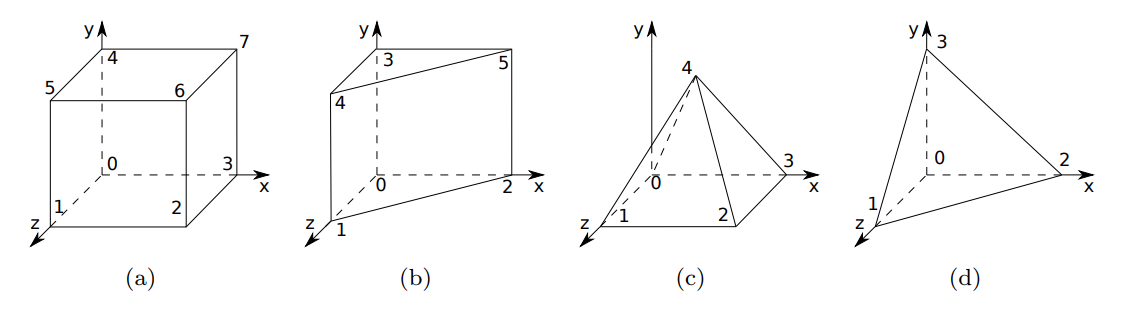
\includegraphics[width=0.95\textwidth]{figures/basic-elements.png}
    \caption{\label{fig:basics_elements} Elementos básicos}
     \small{(a) hexaedro, (b) prisma (cuña), (c) pirámide y (d) tetraedro.} \\
    Fuente: \cite{Gonzalez2014}
\end{figure}

% proceso de division en octantes
Supongamos que $\Omega$ es el dominio de entrada para el que se requiere generar una malla. La mayoría de algoritmos de mallado basados en octantes encapsulan el dominio $\Omega$ en un octante principal o primario y, a continuación, proceden a subdividir recursivamente los octantes hasta que se cumple una determinada restricción, generalmente un delta de error de representación.

El número de subdivisiones recursivas realizadas sobre un octante se denomina nivel de refinamiento ($RL$). Algunos algoritmos ofrecen la posibilidad de definir distintas regiones de refinamiento sobre $\Omega$. Para cada región, puede definirse un $RL$ mínimo y un octante puede pertenecer a varias regiones. Cuando un octante se divide y algunos de sus hijos se sitúan completamente fuera del dominio $\Omega$, su proceso de refinamiento se detiene y se eliminan de la representación.

Un octree equilibrado significa que dos octantes adyacentes no pueden tener una diferencia de nivel de refinamiento superior a uno, como se menciona en \cite{daines2018repairing}. Una malla basada en octantes suele requerir un octree de este tipo. Para ello, algunos octantes se refinan más allá de su $RL$ original. En la Fig.\ref{fig:octree-mesh} se muestra un ejemplo análogo en 2D para ilustrar el proceso de división en 8 hexaedros.

La tarea principal de esta investigación es el refinamiento de las mallas, es decir, aumentar la densidad de nodos que conforman la malla para así aumentar a su vez la definición de la representación. Sin embargo este aumento en la cantidad de nodos no debe ser uniforme en toda la malla ya que afectaría considerablemente el tiempo de ejecución de las simulaciones. Es por esto que algunas técnicas de generación de mallas utilizan refinamiento parcial \cite{lobos2015mixed}, donde son seleccionadas ciertas regiones de la malla en las que se quiere mayor definición y solo dichas zonas de interés son refinadas. En el caso de la figura \ref{fig:octree-mesh}, una malla en 2D de refinamiento parcial, la región de interés es el borde del dominio identificado con el color gris.

\begin{figure}[!ht]
    \centering
    % 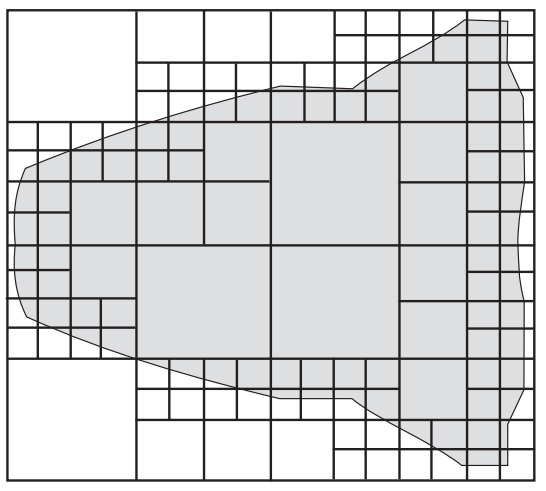
\includegraphics[width=0.5\textwidth]{figures/octree-mesh.png}
    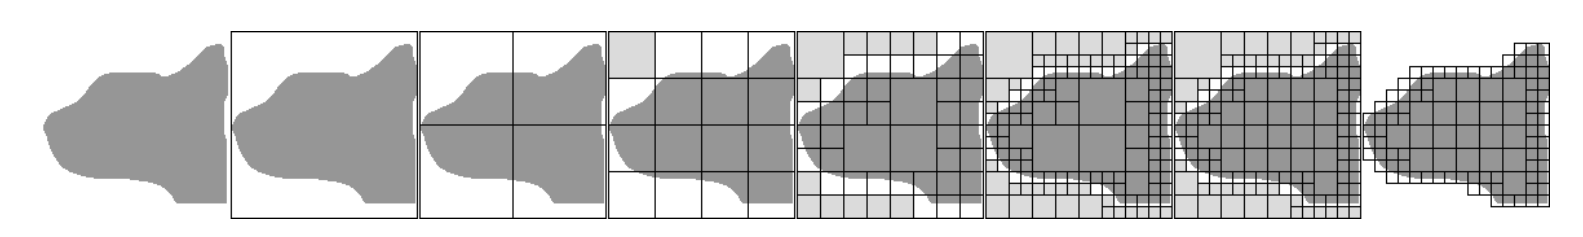
\includegraphics[width=1.0\textwidth]{figures/divison-process.png}
    \caption{\label{fig:octree-mesh} Malla Octree parcialmente refinada.}
    \small{Ejemplo en 2D de la generación de una malla octree equilibrada utilizando un algoritmo basado en Octree.
    Con nivel de refinamiento $RL$ 4 en la región $\Omega$ demarcada con gris. El resto de la malla no tiene definido un $RL$ mínimo, por lo que los octantes que no intersectan con el límite de $\Omega$ tienen su refinamiento detenido.} \\
    Fuente: \cite{lobos2015mixed}
\end{figure}

En una malla al haber distintos niveles de refinamiento, se pueden formar mallas no conformes. 

Un octree equilibrado no es conforme cuando hay múltiples $RL$ y no se respeta la regla de los $RL$ adyacentes. Para mantener la continuidad de la malla, debe aplicarse un patrón de transición sobre los octantes con vecinos de diferentes $RL$. Un patrón de transición sustituirá el hexaedro no conforme por diferentes tipos de elementos, de modo que se garantice que la malla de salida sea conforme. En la Fig. \ref{fig:transition_pattern}  se muestra un ejemplo de patrón de transición.

Una malla es conforme cuando es topológicamente correcta, es decir, tiene todos sus nodos de los bordes y caras consistentes para todos los elementos adyacentes. 

Para construir una malla conforme con refinamiento parcial, se puede hacer uso de elementos especiales que forman transiciones entre regiones con distinto nivel de refinamiento. Este conjunto de elementos se le denomina patrones de transición. En la Fig. \ref{fig:transition_pattern} se puede observar que el elemento B constituye un patrón de transición entre zonas con distinto nivel de refinamiento, en donde el elemento A presenta más refinamiento que el elemento C.

\begin{figure}[!ht]
    \centering
    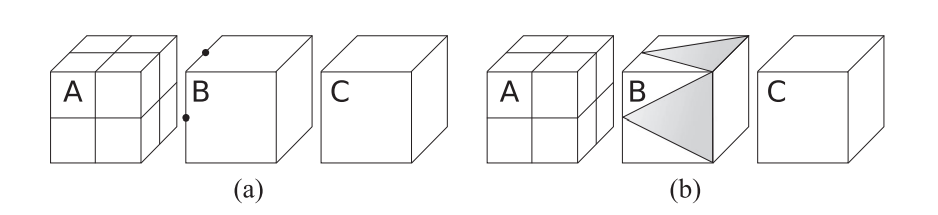
\includegraphics[width=1\textwidth]{figures/transition_pattern_complete.png}
    \caption{\label{fig:transition_pattern} Patrón de transición.} 
    \small{(a) Octante B es el único elemento que requiere un patrón de transición. (b) Malla conforme, topológicamente correcta, resultante de la transición.} \\ Fuente: \cite{lobos2015mixed}.
\end{figure}

La técnica de generación de mallas a utilizar en esta memoria será la técnica que utiliza elementos mixtos para construir patrones de transición.
Dichos elementos son tetraedros, hexaedros, prismas y pirámides de base cuadrada. Todos los patrones existentes fueron diseñados y presentados en \cite{Gonzalez2014}. Además, también hay técnicas que los utilizan para la representación de los bordes en la malla, definiendo un conjunto de elementos, llamados patrones de superficie, que reemplazan los hexaedros encontrados en los bordes.

Algunas mallas de refinamiento parcial pueden verse afectadas negativamente por transiciones entre regiones de diferente nivel de refinamiento en la superficie, llegando muchas veces a invalidar ciertos elementos involucrados. 

% explicación de invalidación
% imagen de elementos invalidados

Aquí se evidencia que los patrones de superficie para generar estas transiciones no están diseñados para ser aplicados sobre elementos mixtos, sino que solamente para mallas compuestas por hexaedros.  Esto puede surgir especialmente en sectores de la malla donde el dominio es cóncavo. 

\subsection{Actualidad}

Actualmente existe un estudio \cite{daines2018repairing} que consiste en reparar elementos inválidos en la superficie de mallas tipo Octree con elementos mixtos y refinamiento parcial. En este estudio se propone una técnica de proyección de nodos para reparar aquellos elementos de los bordes en regiones de transición de la malla, esta técnica se aplica iterativamente debido a que en cada iteración se pueden generar nuevos elementos inválidos.

\subsection{Lineamiento}


% por qué es importante la calidad de los elementos
% cómo se medirá la calidad
% qué es validar la malla
% por qué es importante validar la malla

Se desarrollará desde otra perspectiva la reparación de los elementos inválidos en las regiones de transición que pueden generarse al intentar lograr una representación correcta de los límites.



\subsection{Objetivos}
\subsubsection{Objetivo general}
Ubicar y reparar elementos inválidos o de mala calidad en la superficie de una malla geométrica tridimensional de tipo octree.

\subsubsection{Objetivos específicos}
\begin{itemize}
    \item Validar la malla resultante de la refinación mediante la técnica Octree.
    \item Medir la calidad de la malla generada y refinar los elementos que sean inválidos.
    \item Establecer una estructura de datos que permita volver a un estado anterior de la malla, así en caso de que existan elementos inválidos, permitir volver a un estado válido anterior.
    \item Realizar pruebas para posteriormente comparar tiempos de ejecución con respecto a la versión propuesta en \cite{daines2018repairing}.
\end{itemize}

% Se debe definir el problema, es importante no confundir definir el problema con describir la solución. Por ejemplo: ``diseñar una arquitectura e implementar una plataforma ...'' es una solución, no un problema.

% Algunos elementos que podrían ir en este capítulo son (no es necesario que vayan todos):
% \begin{itemize}
%     \item Breve descripción del contexto donde se realizará la memoria (organización, línea dentro de la Informática en la que se basa, etc.)
%     \item ¿Qué y cómo se realiza actualmente la situación que mejorarás con tu memoria?
%     \item ¿Qué actores o usuarios están involucrados?
%     \item ¿Qué dificultades tienen esos actores actualmente? ¿cuántos son? (ideal si se pueden poner estadísticas para así saber si existe un mercado razonable para la solución que propondrás en tu memoria, en el fondo saber cuántas personas u organizaciones tienen el mismo problema que estás definiendo)
%     \item ¿Qué podría pasar si en el corto o mediano plazo no se solucionan esas dificultades (¿es decir, si no se hiciera tu memoria, qué pasaría?; en el fondo justificar por qué conviene hacer tu memoria, ¿cuál es la motivación o interés de hacerla?).
%     \item ¿Qué competencia existe actualmente? (a lo mejor ya existe una solución al problema, pero por qué no sirve, o por qué tu solución sería mejor, también se puede enfocar a si este problema existe en otras realidades y cómo ha sido solucionado allí).
%     \item Precisar los objetivos y alcances de la memoria (o solución al problema).
% \end{itemize}

% En este capítulo, de ser necesario puede usar referencias bibliográficas (velar porque sean recientes), una cita de ejemplo \cite{schwab2002cure} y otras más \cite{georget1994study,beaumont1990patient}.

% Recuerde poner notas al pie de página que sean explicativas \footnote{Este es un ejemplo de una nota al pie de página. Puede indicar alguna URL, definiciones, aclarar alguna información pertinente del texto, citar algunas referencias, etc..}.

\newpage
\secnumbersection{Marco conceptual}

Los algoritmos basados en la técnica Octree deben gestionar el problema mencionado en la sección anterior, la representación incorrecta de los límites del dominio, por sobre todo en dominios cóncavos.

Un octante límite es aquel que intersecta la frontera de $\Omega$ \footnote{$\Omega$ : dominio de entrada para el que se requiere generar una malla.}, puede presentar nodos dentro y fuera del dominio $\Omega$, los nodos que estén justo en la frontera son considerados nodos externos.

Cuando el octante límite contiene sólo un hexaedro, puede emplearse un patrón de superficie, definidos en \cite{lobos2013patterns}, dicho trabajo presenta un conjunto de patrones de elementos mixtos, que se emplean en la superficie del dominio objetivo y permiten conservar la consistencia de las mallas resultantes, estos patrones están pensados para combinarse con cualquier técnica de mallado que produzca una malla hexaédrica regular o irregular, las mallas Octree son un tipo de malla hexaédrica. Un patrón de superficie es un conjunto de diferentes tipos de elementos que sustituyen al hexaedro para reducir las posibilidades de producir elementos inválidos. Dependiendo de la configuración de nodos internos/externos del octante, se empleará un patrón distinto.

En \cite{lobos2015mixed} se describe una técnica de mallado que incluye patrones de superficie y transición. Esta técnica permite definir diversos $RL$ para $\Omega$. Esta técnica es la base del trabajo desarrollado por Daines y Lobos en \cite{daines2018repairing} y del presente trabajo.

En \cite{daines2018repairing} se detectó que este algoritmo puede producir algunos elementos no válidos cuando las transiciones entre regiones de diferente $RL$ se presentan en el borde. Se trata de un octante que debe llenar ambas regiones, gestionar una transición y, al mismo tiempo lograr la representación del borde. 

\subsection{Medida de calidad para elementos en Mallas Mixtas}

En general, la calidad de un elemento geométrico viene determinada por el nivel de deformación en comparación con la representación geométrica más regular o perfecta del elemento.

La medición de la calidad tiene dos propósitos fundamentales: 

\begin{itemize}
	\item Comparar la malla, ya sea con otras mallas producidas por el mismo dominio o con la propia noción de malla ``teóricamente perfecta".
	\item Mejorarla, es decir, obtener una malla ``mejor'' comenzando por un estado de mala calidad mediante el uso de algoritmos de reparación.
\end{itemize}

% Para el hexaedro, el tetraedro y la cuña se utiliza la variación regular. Por desgracia no existe una variación regula para todas las pirámides. 

Existen múltiples medidas de calidad de los elementos geométricos utilizados, cada una de las cuales mide distintos tipos de deformaciones.
Una medida utilizada habitualmente es la relación de aspecto, $AR$ \footnote{ AR : Aspect Relation.}. En general, el $AR$ de un elemento es la relación entre su borde más corto y su borde más largo. Otra variación significativa es el Relación de Aspecto Gamma, ARG \footnote{ARG: Aspect Ratio Gamma.}, el $ARG$ penaliza más las deformaciones de un tetraedro en comparación con otras variaciones del $AR$.
Para medir la distorsión de un nodo en contraste con su vecino podemos utilizar la \textit{Jacobiana}. Siendo $J^a$ el Jacobiano del nodo $a$ y $d_i$ el vector del nodo $a$ al nodo $i$. El Jacobiano se puede calcular realizando el producto punto entre la distancia nodal del vector altura del tetraedro y el producto cruz de las distancias nodales de los vectores basales.

El problema del Jacobiano es sus dependencias a las distancias entre nodos y a la ortogonalidad entre sus aristas, con respecto a la primera, dos elementos con los mismos ángulos internos pero con tamaños distintos de aristas obtienen distintos valores para esta medida de distorsión y sobre la segunda, la medida de calidad no se puede extender a todos los tipos de elementos geométricos que se encontrarán en las mallas mixtas.

Por tanto, para suplir la dependencia a las distancias se utilizará el Jacobiano Escalado, $J_S$ \footnote{$J_S$ : Scaled Jacobian}.
Esta medida de calidad normaliza los vectores del tetraedro, así sólo dependerá de la ortogonalidad de sus aristas.
El $J_S$ de un hexaedro es el peor $J_S$ de sus nodos. 

En \cite{daines2018repairing} se define el rango de aceptación de la calidad de los elementos. Principalmente, $J_S < 0$ son \elements{} invertidos, se define en \cite{shepherd-2008} un estándar utilizado en las métricas de calidad para Jacobiano Escalado importado por la librería Veredict de Cubit \cite{verdict} que fija $J_S < 0$ como Elementos de inaceptables y $J_{S} \in [0, 0.2[$, correspondería a Elementos cuestionables, es decir, Elementos de calidad deficiente. Además, se destaca el estándar de ANSYS, una herramienta robusta a la hora de realizar simulaciones computarizadas, que considera $J_{S} \in [0, 0.03[$, como Elementos inválidos. Elementos con $J_S \geq 0.2$ como Elementos de buena calidad y Elementos con $J_{S} = 1$, como un hexaedro perfecto.

%
Por tanto, para este análisis se acotará definiendo $J_{S} \in ]-1, 0]$ como \elements{} inválidos, estos específicamente corresponden a \elements{} negativos o invertidos, que conformarían mallas con topología inconsistente. Luego, se considerará, a diferencia de los trabajos anteriores, \elements{} de calidad cuestionable los que presenten $J_{S} \in ]0, 0.05]$, este intervalo se acotará y separará en dos intervalos, $J_{S} \in ]0, 0.03] \wedge J_{S} \in ]0.03 , 0.05]$, esto con el fin de enfocar el estudio en \elements{} que produzcan una malla inconsistente, reduciendo la cota superior de $0.2$ a $0.05$ y estudiar las consecuencias en la propagación del cambio de la calidad del refinamiento, dividiendo el intervalo en dos, considerando el estándar de ANSYS como referencia al dividir dicho intervalo.

%Además, se definirá la frecuencia de Elementos con $J_{S} \in ]m, n]$ , como $E^{n}_{m}$.
%
%Entonces, se graficará en \autoref{fig:fit_all_bar}, los histogramas de cada malla para los intervalos definidos por $EC$.
%Teniendo, $E^{0}_{-inf}$, $E^{0.03}_{0}$, $E^{0.05}_{0.03}$, como los intervalos a estudiar, en $E^{0}_{-inf}$ se refleja la cantidad de Elementos por refinar en cada iteración, analizado anteriormente en el ajuste.
% Más adelante se establecerán diferentes estandares para identificar elemementos inválidos


Por otra parte, para suplir la deficiencia en su dependencia a la ortogonalidad de sus aristas, se usará un Jacobiano para cada uno de los tipos de elementos que encontraremos en la malla, esta medida de calidad es el Jacobiano Escalado Normalizado del Elemento \footnote{$J_{ENS}$ : Element Normalized Scaled Jacobian}, más adelante denotado como $J_{ENS}$.


El indice $J_{ENS}$ calcula el $J_S$ del elemento perfecto $K^e$, donde $e$ denota el elemento correspondiente. Los valores para los distintos elementos utilizados en este trabajo para las mallas Octree mixtas se encuentran en la siguiente \autoref{eq:const_jens}.


\begin{equation} \label{eq:const_jens}
    \begin{aligned}
    K^T &= \frac{\sqrt{2}}{2} \longrightarrow \text{Tetraedro} \\
    K^P &= \frac{\sqrt{6}}{3} \longrightarrow \text{Pirámide} \\
    K^W &= \frac{\sqrt{3}}{2} \longrightarrow \text{Cuña}
    \end{aligned}
\end{equation}

De esta forma, como se vio en \cite{daines2018repairing}, con ayuda de estas constantes podemos calcular el $J_{ENS}$ de cualquier nodo de un elemento sustituyendo el valor correspondiente en la \autoref{eq:node_jens}. De forma similar a $J_S$ para realizar el cálculo de $J_{ENS}$ utilizamos la \autoref{eq:jens}, donde $i$ son los nodos del elemento $e$. y $J^e_{ENS}$ es su $J_{ENS}$.

\begin{equation} \label{eq:node_jens}
    \begin{aligned}
J^n_{ENS} &=    
\left\{
\begin{array}{rl}
     ( 1 + K^e ) - J_S, & \qquad J_S > k^e
  \\ Js/K^e, & \qquad -k^e \leq J_S \leq K^e
  \\ -( 1 + K^e ) - J_S, & \qquad J_S < -k^e
\end{array}
\right.
    \end{aligned}
\end{equation}


\begin{equation} \label{eq:jens}
    \begin{aligned}
J^e_{ENS} &=    
\left\{
\begin{array}{ll}
     \text{min}\{J^i_{ENS}\}, & \qquad \forall i, J^i_{ENS} > 0
  \\ \text{max}\{J^i_{ENS}\} : J^i_{ENS} < 0, & \qquad \exists i, J^i_{ENS} < 0
\end{array}
\right.
    \end{aligned}
\end{equation}

% mallas octree
% elementos invalidos
% patrones de transición
% explicación del algoritimo 
% explicación de la tecnica de generación de mallas
% explicación de la tecnica de refinamiento
% explicacción de la tecnica de reparación
% explicación de la tecnica de selección del elemento invalido
% explicación de la herramienta usada


% Se debe describir la base conceptual o fundamentos en los que se basa tu memoria, es decir, todos los conceptos técnicos, metodologías, herramientas, etc. que están involucradas en la solución propuesta. En el fondo esta parte permite precisar y delimitar el problema, estableciendo definiciones para unificar conceptos y lenguaje y fijar relaciones con otros trabajos o soluciones encontradas por otros al mismo problema evitando así plagios o repetir errores ya conocidos o abordados por otros.

% En esta parte es importante relacionar estos conceptos con la memoria y es fundamental utilizar referencias bibliográficas (o de la web) recientes, por ejemplo \cite{gettelfinger2004will}.


Para $J_{ENS}$ se definen los mismo intervalos que para $J_S$ para identificar Elementos.

\begin{itemize}
	\item $J_{ENS} \in ]-1, 0]$ : Elementos inválidos.
	\item $J_{ENS} \in ]0, 0.05]$ : Elementos cuestionables.
	\item $J_{ENS} \in ]0.05, 1]$ : Elementos de buena calidad.
\end{itemize}

En la etapa de validación, el estudio se concentrará en contabilizar la frecuencia de \elements{} que presentan una calidad no deseable(inválidos y cuestionables), por ello se definirá la frecuencia de Elementos con $J_{ENS} \in ]m, n]$ , como $E^{n}_{m}$.

Teniendo, $E_{-1}^{0}$, como la expresión que se referirá a la frecuencia de \elements{} Inválidos, $E_{0}^{0.03}$, a los \elements{} Cuestionables y $E_{0.03}^{0.05}$, a parte de los \elements{} de Buena Calidad
% Más adelante se establecerán diferentes estandares para identificar elemementos inválidos


\subsection{Malla inicial}

Para comprender de mejor forma el problema buscaremos un entorno donde existan elementos inválidos, para ello procederemos a estudiar la localidad de los elementos de mala calidad, entonces se generará una malla que llamaremos la \textit{malla inicial}.

Ésta será la representación de una corteza cerebral a un nivel 5 de refinamiento en general y se le aplicará un refinamiento de nivel 7 a una superficie prismática regular inserta en la parte frontal del cerebro. Como se muestra en la representación de puntos de la malla del cerebro y representación alámbrica de la superficie prismática de la \autoref{fig:cortex_surf}.

\begin{figure}[H]
    \centering
    \begin{subfigure}[t]{0.45\textwidth}
        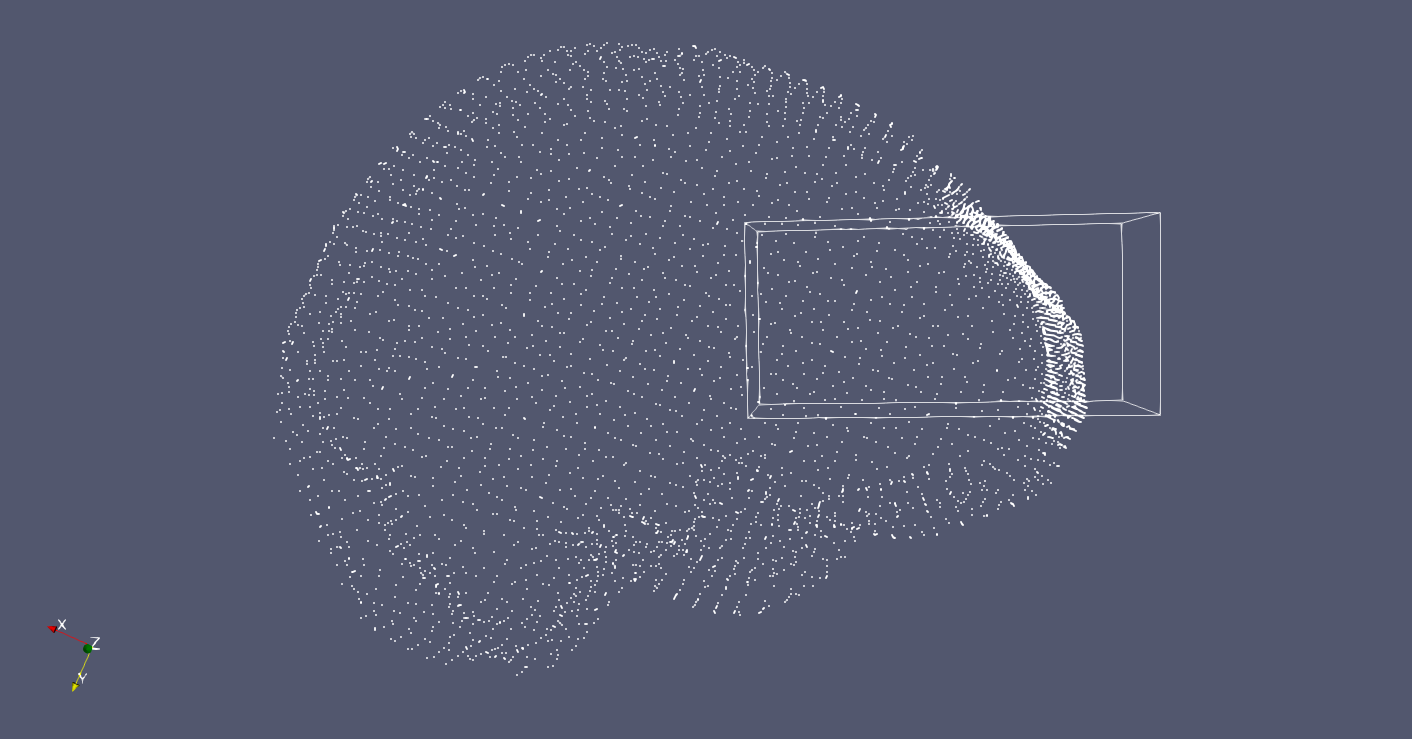
\includegraphics[width=1.0\textwidth]{figures/bad_quality_zone/cortex_surf.png}
        \caption{Perspectiva lateral}
    \end{subfigure}
    \begin{subfigure}[t]{0.45\textwidth}
        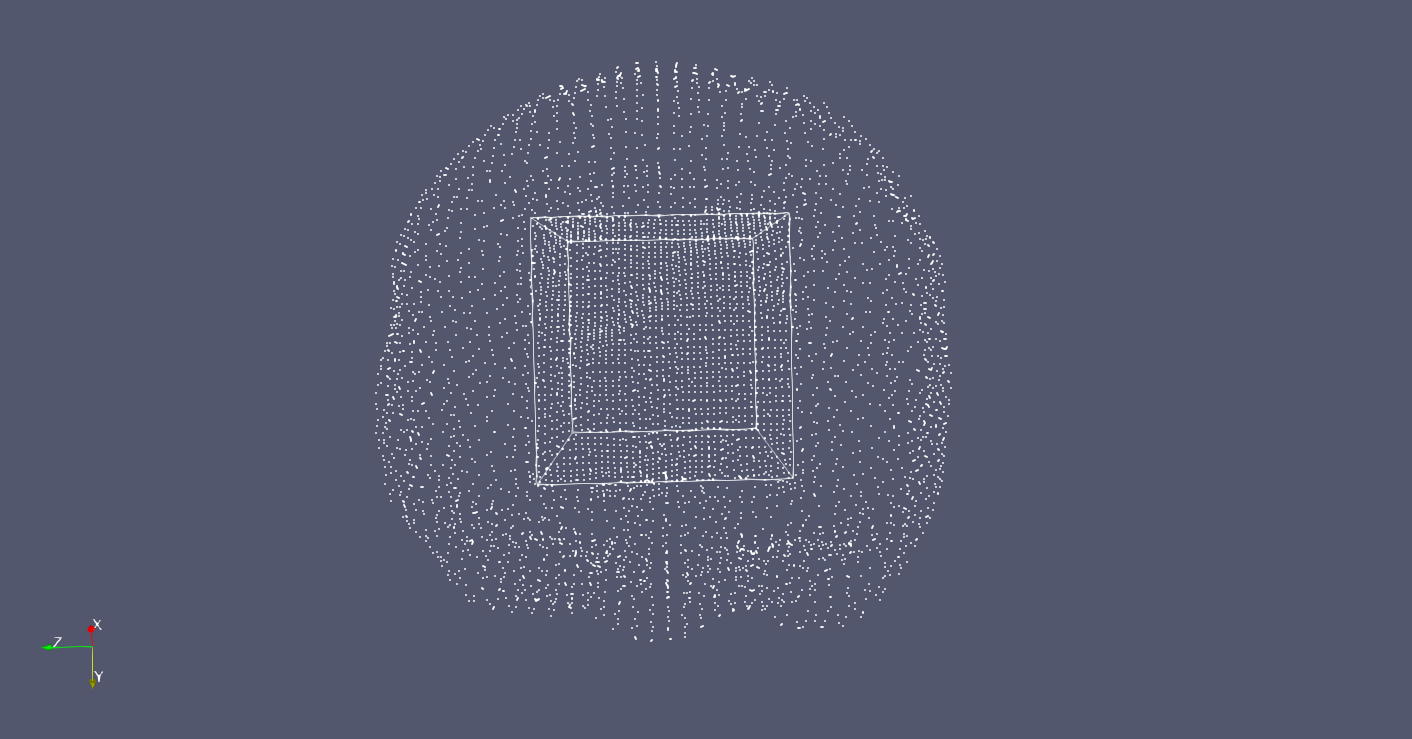
\includegraphics[width=1.0\textwidth]{figures/bad_quality_zone/cortex_surf_points.png}
        \caption{Perspectiva frontal}
    \end{subfigure}
    \caption{  Muestra frontal y lateral de la malla inicial con refinamiento global de nivel 5 y refinamiento en superficie prismática regular de nivel 7.\\ Fuente: Elaboración propia.}
    \label{fig:cortex_surf}
\end{figure}

\subsection{Herramientas}

En este trabajo se utilizarán algunas herramientas construidas por la comunidad como el generado de Mallas, el generador de estadísticas $J_{ENS}$, un software para visualización, scripts en Bash y Python para la ejecución de la solución y el análisis de los resultados, respectivamente.

\subsubsection{Mixed-element mesh generator} \label{section:mesh_generator_definition}

El generador de mallas de elementos mixtos \cite{lobos2015mixed} es una herramienta creada para facilitar la generación de mallas, a través de la linea de comandos se puede generar mallas con superficies de refinamiento en diferentes niveles, exportar en diversos formatos para visualización, iniciar con una malla refinada y refinar específicamente octantes entregados como input.
Este software recibe modelos de datos de mallas en formato \textit{mdl}.

\begin{lstlisting}[style=Console,caption={Opciones de mesher generator.\\ Fuente: Elaboración propia.}]
input  >    ./mesher -h
output >    use:  ./mesher [-d] input.mdl [-o] input.off [-u] output
                    [-c] volume_mesh.oct (octant mesh to start from)
                    [-s] ref_level [-a] ref_level [-b] file.reg 
                    [-l] list_file.txt [-r] input_surface rl [-g] [-v]
            where:
              one of the parameters must be an input surface mesh in
              mdl or off format. If output name is not provided it
              will be saved in input_name.m3d. Options:
                -s Refine octants intersecting the input surface.
                   Parameter ref_level is the refinement level
                -a Refine all elements in the input domain.
                   Parameter ref_level is the refinement level
                -b Refine block regions provided in file file.reg
                -l Refine elements provided in the file by their index
                -r Refine surface region. Will refine all the elements
                   in the provided input_surface at level rl
                -g save output mesh in GetFem format (gmf)
                -v save output mesh in VTK ASCII format (vtk)
                -i save output mesh in MVM ASCII format (mvm)
                -m save output mesh in M3D ASCII format (m3d)
\end{lstlisting}

Se denominará como \textit{MESHER\_GENERATOR} en el resto del presente trabajo.

De esta herramienta, se destacará los diferentes formatos de exportación:

\begin{itemize}
	\item vtk: Formato utilizado para visualización en la plataforma Paraview.
	\item oct: Formato utilizado para persistir los datos utilizados en el algoritmo.
\end{itemize}

Adicionales a estos formatos, se agregarán algunos importantes adicionales para realizar las iteraciones y validaciones correspondientes explicados en la siguiente sección.

Otra funcionalidad a destacar es la opción de refinamiento dado un listado de Octantes y Elementos, que se explotará y mejorará para definir esta propuesta.

\subsubsection{Mixed-element $J_{ENS}$ stadistics generator}

El generador de estadísticas $J_{ENS}$ para mallas Octree de elementos mixtos es una herramienta que facilita la validación de mallas, creada por la comunidad y liderado por el profesor Claudio Lobos. Puede generar histogramas con diferentes índices como Scaled Jacobian, Normalized Scaled Jacobian, Aspect Ratio, etc. 
En este trabajo lo utilizaremos principalmente para validar cada malla generada enfocándonos sólo en obtener la frecuencia del indice $J_{ENS}$. Esto es un histograma con la frecuencia de todos los elementos de la malla con $J_{ENS} \in \{-1 , 1\}$, como se muestra en la figura \autoref{out:jens_output_c_5r7_0}.

\begin{lstlisting}[style=console,caption={Opciones de jens calculator. \\ Fuente: Elaboración propia.}]
input   >   ./jens -h
output  >   use: ./jacobian -option input.m3d
            options:
            -s : Scaled Jacobian statistics
            -e : Element Normalized Scaled Jacobian statistics
            -j : List Jens of each Element Jens [Js]
            -a : List Aspect Ratio for each element
            -l : List Jens of each node for each element
\end{lstlisting}


\begin{lstlisting}[style=console,label={out:jens_output_c_5r7_0},caption={Estadísticas Jens para malla inicial, muestra una lista de frecuencias para diferentes cotas superiores para la calidad Jens encontrada en la malla.\\ Fuente: Elaboración propia.}]
input   >   ./jens -e ./src/c_5r7.mdl
output  >   negative: 27
            <0.0333 : 4
            <0.05   :5
            <0.1    :13
            <0.15   :54
            <0.2    :219
            <0.25   :356
            <0.3    :9918
            <0.35   :8431
            <0.4    :3386
            <0.45   :6641
            <0.5    :2341
            <0.55   :16891
            <0.6    :2659
            <0.65   :2689
            <0.7    :2038
            <0.75   :4872
            <0.8    :1108
            <0.85   :2477
            <0.9    :457
            <0.95   :408
            <1      :108662
            total: 173656
            worst quality -0.792707
            average quality 0.806127
\end{lstlisting}

Se denominará como \jens{} el resto del presente trabajo.

Convenientemente, los primeros tres intervalos del histograma pertenecen a los intervalos de interés para este estudio.

\subsubsection{ParaView}

Paraview es un software open-source multiplataforma que facilita la visualización de representaciones en 3D. Presenta una interfaz interactiva, nos ayudará analizar visualmente el estado de la malla en todo momento. Se utilizará el formato con extensión \textit{vtk} para visualizar mallas en esta plataforma.

Este software presenta diferentes secciones que nos ayudarán a analizar cada malla generada, la sección marcada con el número 1 en \autoref{fig:paraview_all}, se presentan todas las mallas que se representarán gráficamente en la sección 2. Existe un panel de herramientas en la sección 3 que nos ayudará a marcar/desmarcar elementos o puntos en el panel 2 que se verán reflejados e identificados en el recuadro 5.
En la sección 4 podremos cambiar la forma de visualizar cada representación, esto nos ayudará a identificar elementos, identificar gráficamente si una malla es válida en su construcción, etc.

\begin{figure}[H]
    \centering
    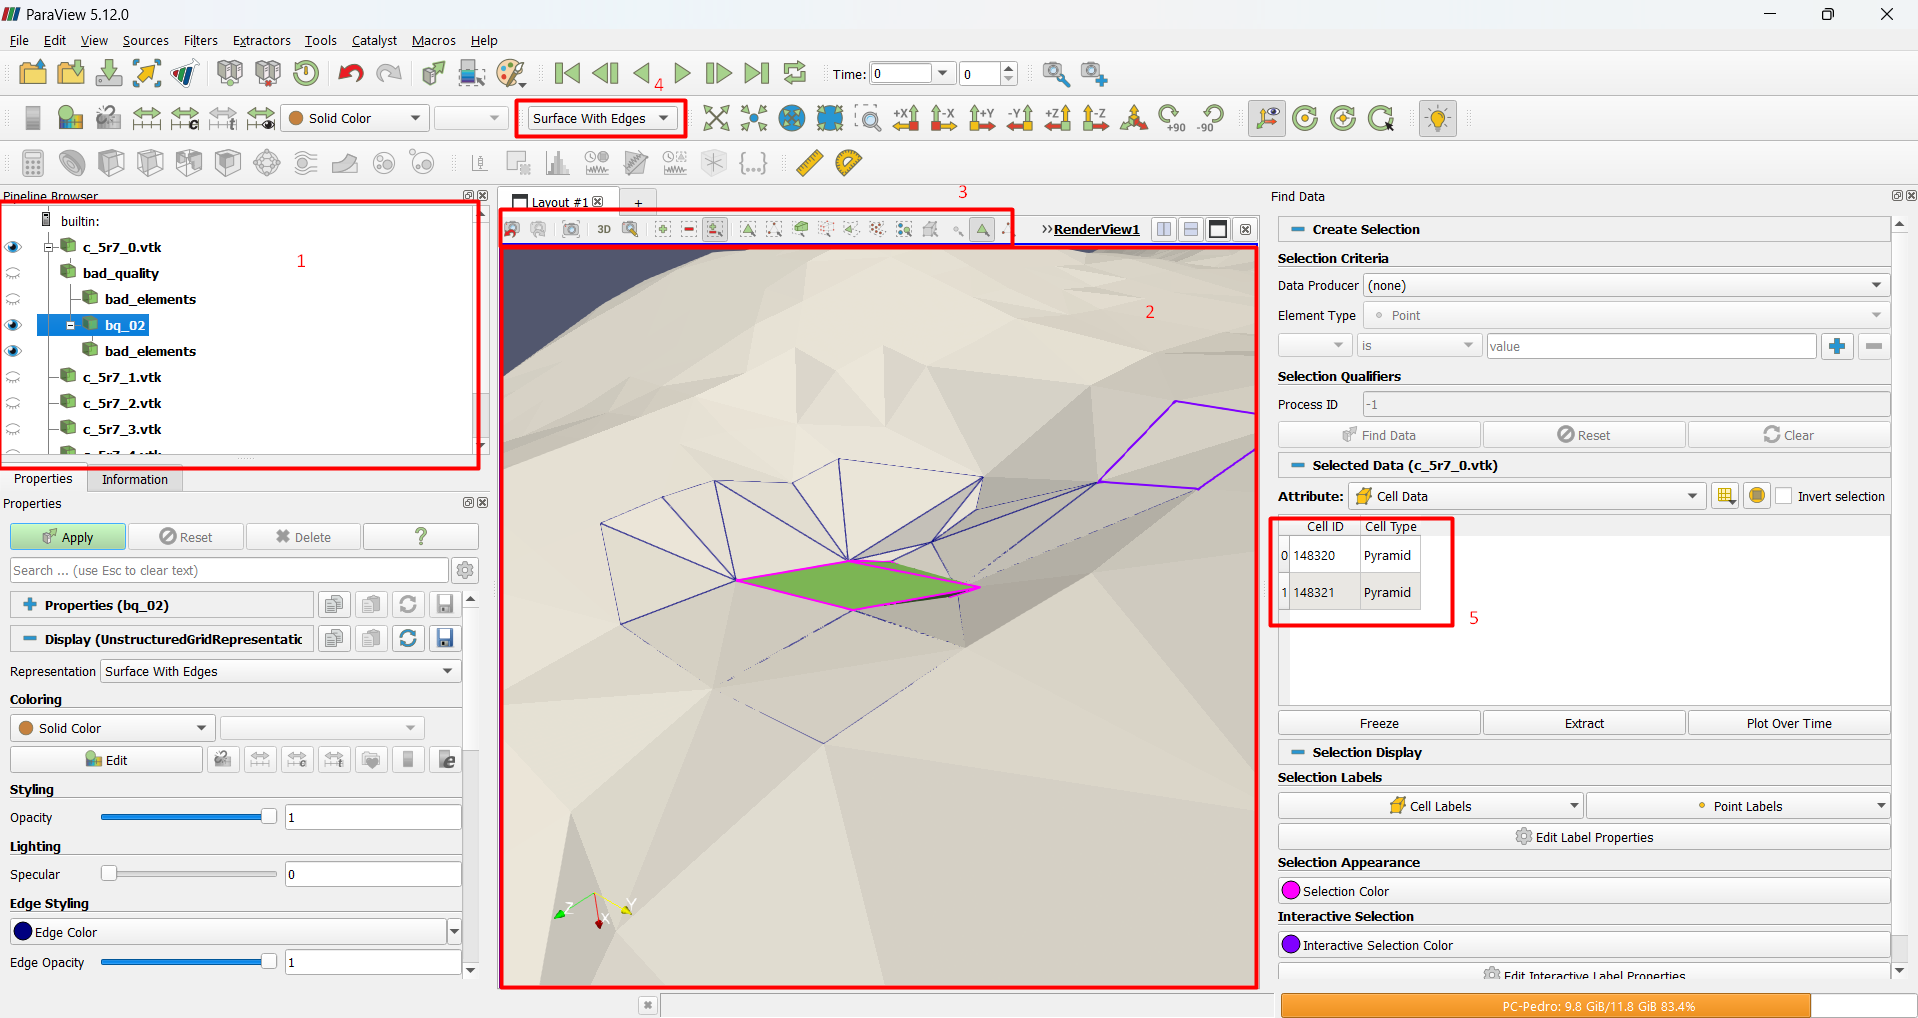
\includegraphics[width=1.0\textwidth]{figures/paraview/paraview_all.png}
    \caption{ Interfaz de software Paraview, se muestra una sección de la malla inicial con dos elementos seleccionados.\\  Fuente: Elaboración propia.}
    \label{fig:paraview_all}
\end{figure}

\subsection{Estructura de datos}

En la construcción de la solución existen diversas estructuras de datos que se van complejizando a medida que se avanza en el algoritmo.

En esta sección sólo se explicará la estructura de datos elemental y de forma general. 

Como se definió anteriormente, una malla Octree se divide en octantes, cada uno de estos octantes contienen Elementos mostrados en la \autoref{fig:basics_elements}.  Luego, cada uno de estos Elementos está constituido por Puntos, que es la unidad más pequeña.

Para ejemplificar en \autoref{fig:entity_relation_diagram}, se presenta un pequeño diagrama entidad relación que muestra la estructura de los objetos relacionados en el algoritmo de la generación de mallas.


%\begin{lstlisting}[style=CStyle,caption={Clase Octant.\\ Fuente: Elaboración propia.},label={code:octant_class}]
%#include <vector>
%class Octant
%{
%	public:
%        Octant(vector<unsigned int> &epts, const unsigned short &ref_level,
%    			   const unsigned int &o_id);
%        ...
%        // indice del octante.
%        unsigned int id;
%        // indices de puntos que conforman al octante.
%        vector<unsigned int> points_indexes;
%        // indices de puntos que conforman los elementos 
%        // pertencientes al octante.
%        vector<vector<unsigned int>> sub_elements_points_indexes;
%}
%\end{lstlisting}

\begin{figure}[H]
	\centering
	\includegraphics[width=0.65\textwidth]{figures/entity_relation_diagram.png}
	\caption{Diagrama entidad-relación de generador de mallas.\\  Fuente: Elaboración propia.}
	\label{fig:entity_relation_diagram}
\end{figure}

\subsubsection{Acercamiento al algoritmo de Mixed-element mesh generator}

Parte importante del software mencionado en la \autoref{section:mesh_generator_definition} es la generación de la malla que se define y explica brevemente en \cite{daines2018repairing}.


\begin{algorithm}[H]
\SetKwInOut{KwIn}{Input}
\SetKwInOut{KwOut}{Output}
% functions
\SetKwFunction{generateMesh}{GENERATE\_MESH}
\SetKwFunction{generateBalancedOctree}{GENERATE\_BALANCED\_OCTREE}
\SetKwFunction{applyTransitionPatterns}{APPLY\_TRANSITION\_PATTERNS}
\SetKwFunction{applySurfacePatterns}{APPLY\_SURFACE\_PATTERNS}
\SetKwFunction{projectOnto}{PROJECT\_ONTO}
\SetKwFunction{add}{ADD}
\SetKwFunction{getBoundaryNodes}{GET\_BOUNDARY\_NODES}
% procedure
\SetKwProg{myproc}{Procedure}{:}{}
\KwIn{Refinement level constraints $RLC$, triangular surface mesh \Omega.}
\KwOut{Volumetric mesh of \Omega that meets $RLC$.}
\myproc{\generateMesh{RLC, \Omega}}
{
    $mesh$ \gets \generateBalancedOctree{RLC,\Omega}\;
    $mesh$ \gets \applyTransitionPatterns{mesh}\;
    $bnodes$ \gets \getBoundaryNodes{mesh, \Omega}\;
    \For{ \textbf{each} $node$ \textbf{in} $bnodes$} {
        \If{$node \in l$ \textbf{or} ($node$ is \textbf{inside} of \Omega\, \& $node$ is \textbf{close} to \Omega)} {
            $node$.\projectOnto{\Omega}\;
        }
    }
    $mesh$ \gets \applySurfacePatterns{mesh}\;
    $bnodes$ \gets \getBoundaryNodes{mesh, \Omega}\;
    \For{\textbf{each} $node$ \textbf{in} $bnodes$} {
        \If{$node$ is \textbf{outside} of \Omega} {
            $node$.\projectOnto{\Omega} \;
        }
    }
    \KwRet mesh\;    
}
\caption{Algoritmo de generación de mallas Octree con elementos mixtos y varios niveles de refinamiento.\\ Fuente: \cite{daines2018repairing}}
\label{alg:propuesta_daines} 
\end{algorithm}

En términos simples,  el algoritmo consiste en generar una malla balanceada Octree, aplicar patrones de transición entre Octantes con diferencias de $RL$ mayor a 1, luego se realizan proyecciones en los nodos que se encuentran cerca de la frontera de $\Omega$ para generar una mejor representación del borde.

Para este estudio, no es necesario profundizar en este algoritmo, pero es importante mencionarlo y entender su estructura de datos para explicar brevemente los diferentes formatos de exportación del algoritmo que utilizaremos para aplicar una versión iterativa del mismo enfocándonos específicamente en los Elementos de mala calidad.




\newpage
\secnumbersection{Propuesta de solución}

\subsection{Comprensión del problema}

Inicialmente sabemos que los elementos inválidos podrían encontrarse luego de refinar una malla Octree con diferentes niveles de refinamiento, específicamente en el límite donde se producen las transiciones entre regiones de diferente nivel de refinamiento.

%Estos elementos inválidos se identificarán por su $J_{ENS}$ menor a cero.
Entonces, se escogerá una malla frecuentemente utilizada en la comunidad, la malla de corteza cerebral, una malla de geometría suficientemente compleja por presentar múltiples concavidades y de calidad de representación suficiente por su amplia densidad de puntos que la conforman, en total $12,986$ puntos, con esta malla se busca realizar un estudio gráfico preliminar.

\subsubsection{Estudio preliminar}

Para comenzar, se debe comprender el alcance del problema, entonces se ejecutó \jens{} a la ``malla inicial'' y se obtuvo el histograma con las estadísticas de calidad de los elementos de la malla inicial, \autoref{out:jens_output_c_5r7_0}.

Nos enfocaremos sólo en elementos inválidos, por lo tanto, el threshold a estudiar será cero en esta etapa previa.

Actualmente, se identificaron 27 elementos invertidos, pero aún no se ha determinado cuáles son específicamente esos elementos. Para resolver este problema, es necesario que el algoritmo \mesher{} incluya una funcionalidad para etiquetar los elementos inválidos.

Para ello se realizó una pequeña modificación a \mesher{}, se le añadieron ciertas funcionalidades de \jens{}, para que al finalizar el proceso de proyección de nodos, calcule el $J_{ENS}$ de cada \element{} presente en cada \octant{} e identifique cuáles son peores que el threshold definido para esta etapa.


% y al final de su algoritmo, cuando se exportan los datos de la malla, en específico, cuando guardan los puntos, elementos y octantes de la malla, se realiza una identificación de los índices de elementos que pertenecen a cada octante y se guardan en su clase como información del octante.

%Para guardarlo en el octante se agrega un atributo a la clase llamado \textit{sub\_elements\_indexes}, línea 16 en \autoref{code:octant_class_modification}.
%
%Este atributo es consultado después, cuando se etiqueta cada octante que presente elementos inválidos.
%
%\begin{lstlisting}[style=CStyle,caption={Modificación Clase Octant.\\ Fuente: Elaboración propia.},label={code:octant_class_modification}]
%#include <vector>
%class Octant
%{
%	public:
%        Octant(vector<unsigned int> &epts, const unsigned short &ref_level,
%    			   const unsigned int &o_id);
%        ...
%        // indice del octante.
%        unsigned int id;
%        // indices de puntos que conforman al octante.
%        vector<unsigned int> points_indexes;
%        // indices de puntos que conforman los elementos 
%        // pertencientes al octante.
%        vector<vector<unsigned int>> sub_elements_points_indexes;
%        // indices de elementos pertenecientes al octante.
%        vector<unsigned int> sub_elements_indexes; 
%}
%\end{lstlisting}


Se propone, de manera similar a \cite{daines2018repairing}, implementar un marcador para los octantes que contengan elementos de mala calidad, basado en una cota superior predefinida, como se muestra en \autoref{alg:get_labeled_octants}.

% Se propone, de manera similar a \cite{daines2018repairing}, un marcador de octantes que contienen elementos de mala calidad dada una cota superior, \autoref{alg:get_labeled_octants}.

Esta técnica permitirá identificar los octantes que necesitan ser refinados en etapas posteriores. En esta fase, nos enfocamos en identificar los elementos contenidos dentro de estos octantes.

Así, al obtener la lista de octantes involucrados, ahora es posible obtener los índices de los elementos que los componen, permitiendo su posterior análisis.


\begin{algorithm}
\caption{Algoritmo para etiquetar octantes que contienen elementos con peor calidad que la cota entregada.}\label{alg:get_labeled_octants} 
\SetKwInOut{KwIn}{Input}
\SetKwInOut{KwOut}{Output}
% functions
\SetKwFunction{getLabeledOctants}{GET\_LABELED\_OCTANTS}
\SetKwFunction{calculateJens}{CALCULATE\_JENS}
\SetKwFunction{getOctant}{GET\_OCTANT}
\SetKwFunction{getIndex}{GET\_INDEX}
\SetKwFunction{add}{ADD}
% procedure
\SetKwProg{myproc}{Procedure}{:}{}
\KwIn{Refinement level constraints $RLC$, triangular surface mesh \Omega, quality threshold $T$, maximum number of iterations $I$.}
\KwOut{if successful, volumetric mesh of \Omega that meet the $RLC$ with quality greather than $T$.}
\myproc{\getLabeledOctants{$M$, $T$}}
{
    $lo$ \gets \, $empty set$ \;
    \For{ \textbf{each} $element$ \textbf{in} $M$} {
        $q$ \gets \, \calculateJens{$element$}\;
        \If{$q < T$} {
            $octant$ \gets \, $element$.\getOctant{}\;
            $octant\_index$ \gets \, $octant$.\getIndex{}\;
            $lo$.\add{$octant\_index$}\;
        }
    }
    \KwRet $lo$\;    
}
\end{algorithm}

Utilizando la lista de elementos involucrados, podemos visualizar los resultados en ParaView. Esto nos permite generar la \autoref{fig:cortex_surf_oct_labeled}, donde los elementos pertenecientes a los octantes afectados se destacan en color verde. 

Con esta visualización, podemos confirmar que estos elementos se encuentran en la vecindad de las transiciones entre regiones con distintos valores de $RL$. Esta representación gráfica facilita la identificación de las áreas problemáticas dentro de la malla y demuestra cómo las transiciones entre regiones con diferentes características influyen en la calidad de los elementos.

% \begin{algorithm}
% \caption{Modificación del algoritmo para etiquetar octantes, permite imprimir en consola los elementos que forman cada octante etiquetado.}\label{alg:get_labeled_octants_modification} 
% \SetKwInOut{KwIn}{Input}
% \SetKwInOut{KwOut}{Output}
% % functions
% \SetKwFunction{getLabeledOctants}{GET\_LABELED\_OCTANTS}
% \SetKwFunction{calculateJens}{CALCULATE\_JENS}
% \SetKwFunction{getOctant}{GET\_OCTANT}
% \SetKwFunction{getIndex}{GET\_INDEX}
% \SetKwFunction{getSubElementIndexes}{GET\_SUB\_ELEMENTS\_INDEXES}
% \SetKwFunction{add}{ADD}
% \SetKwFunction{size}{SIZE}
% % procedure
% \SetKwProg{myproc}{Procedure}{:}{}
% \KwIn{Malla Octree $M$, cota de calidad $T$.}
% \KwOut{Lista de Octantes con elementos de mala calidad etiquetados.}
% \myproc{\getLabeledOctants{$M$, $T$}}
% {
%     $lo$ \gets \, empty set \tcp*{Lista de Octantes etiquetados.} 
%     \For{ \textbf{each} $element$ \textbf{in} $M$} {
%         $q$ \gets \, \calculateJens{$element$}\;
%         \If{$q < T$} {
%             $octant$ \gets \, $element$.\getOctant{}\;
%             $octant\_index$ \gets \, $octant$.\getIndex{}\;
%             $lo$.\add{$octant\_index$}\;
%             $le$ \gets \, $octant$.\getSubElementIndexes{}\;
%             \textbf{PRINT} octant: $octant\_index$ \;
%             \textbf{subelements:} \;
%             \For{ $k \gets 0$ to $le$.\size{} } {
%                 \textbf{PRINT} $le_{k}$
%             }
%         }
%     }
%     \KwRet $lo$\;    
% }
% \end{algorithm}

\begin{figure}[!ht]
    \centering
    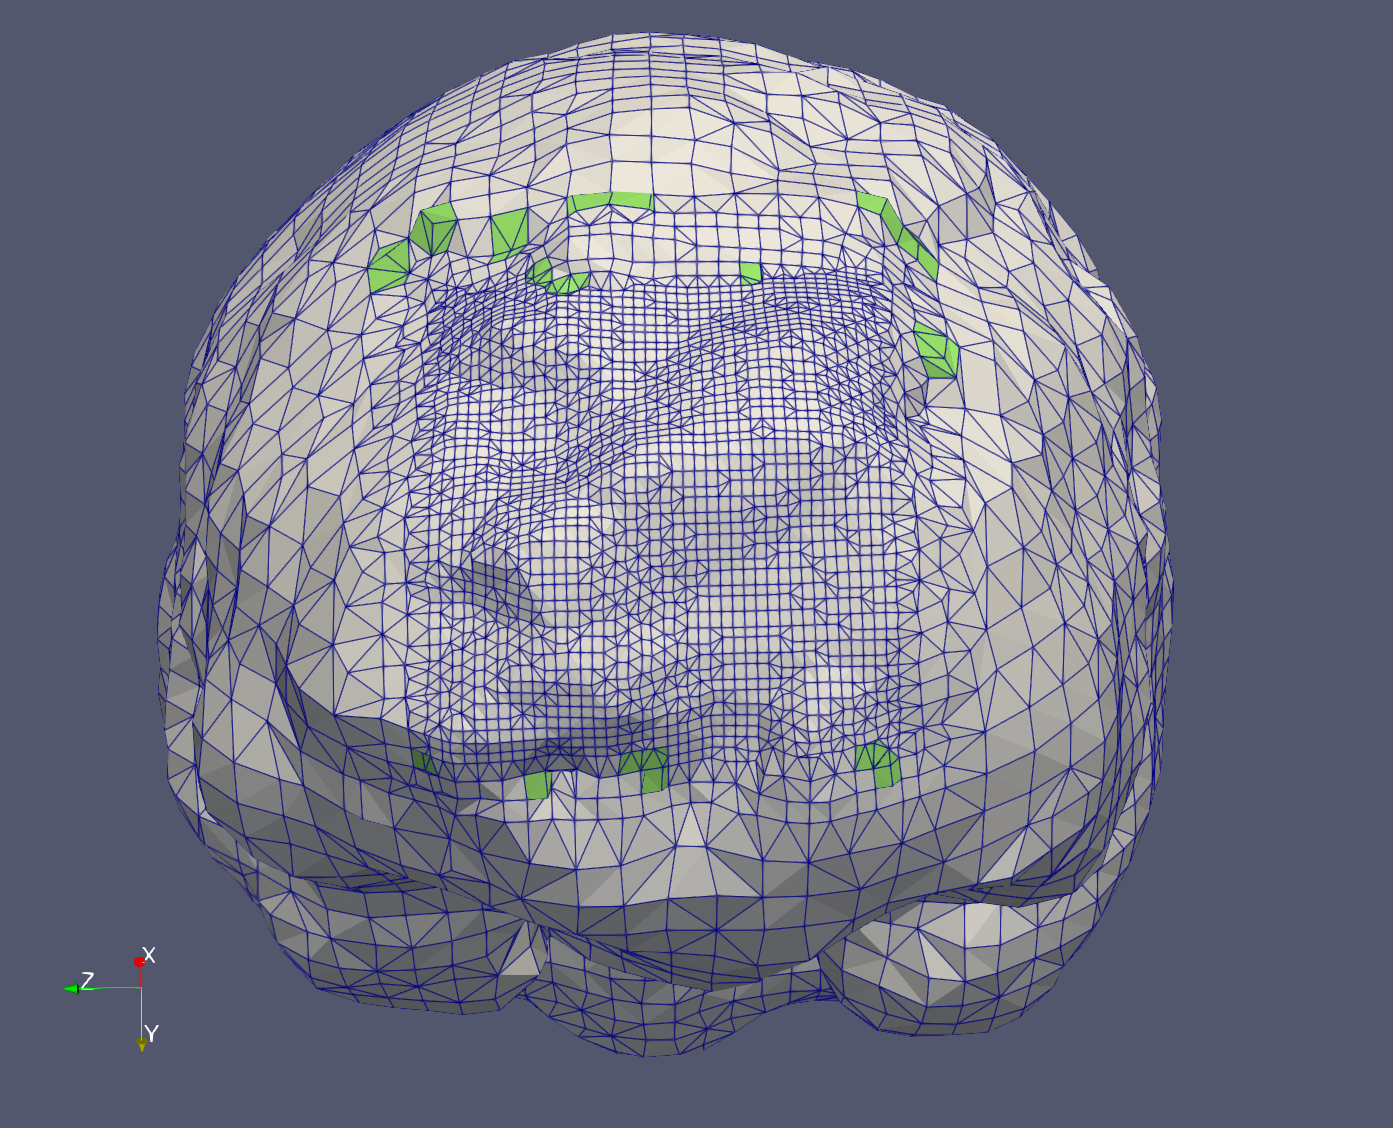
\includegraphics[width=0.6\textwidth]{figures/labeled_octs/labeled_oct_c_5r7_0.png}
    \caption{ Zona frontal de la malla donde se presentan los elementos inválidos (verde). }
    Fuente: Elaboración propia.
    \label{fig:cortex_surf_oct_labeled}
\end{figure}

\subsubsection{Comprensión de elementos inválidos}

Para comprender la naturaleza de los elementos invertidos, se realizará un análisis gráfico localizado, centrándose en un octante específico situado en la parte inferior izquierda del frontis de la malla. Este octante ha sido seleccionado debido a su característica cóncava en la superficie y porque contiene varios elementos inválidos. Además, se encuentra en la intersección de dos regiones que requieren refinamiento, cada una con diferentes valores de $RL$.

En la \autoref{fig:zoom_cortex_surf}, se presenta la región de interés en el contexto de la malla inicial. La imagen a la izquierda muestra el lóbulo frontal con la zona a estudiar en color celeste, incluye todos los \elements{} del \octant{}, mientras que la imagen a la derecha proporciona una vista ampliada de la zona aislada del \octant{} afectado, la zona en celeste. En esta vista detallada, se pueden observar solo los \elements{} contenidos en dicho \octant{}, con los \elements{} inválidos resaltados en verde.

\begin{figure}[!ht]
    \centering
    \begin{subfigure}[t]{0.45\textwidth}
        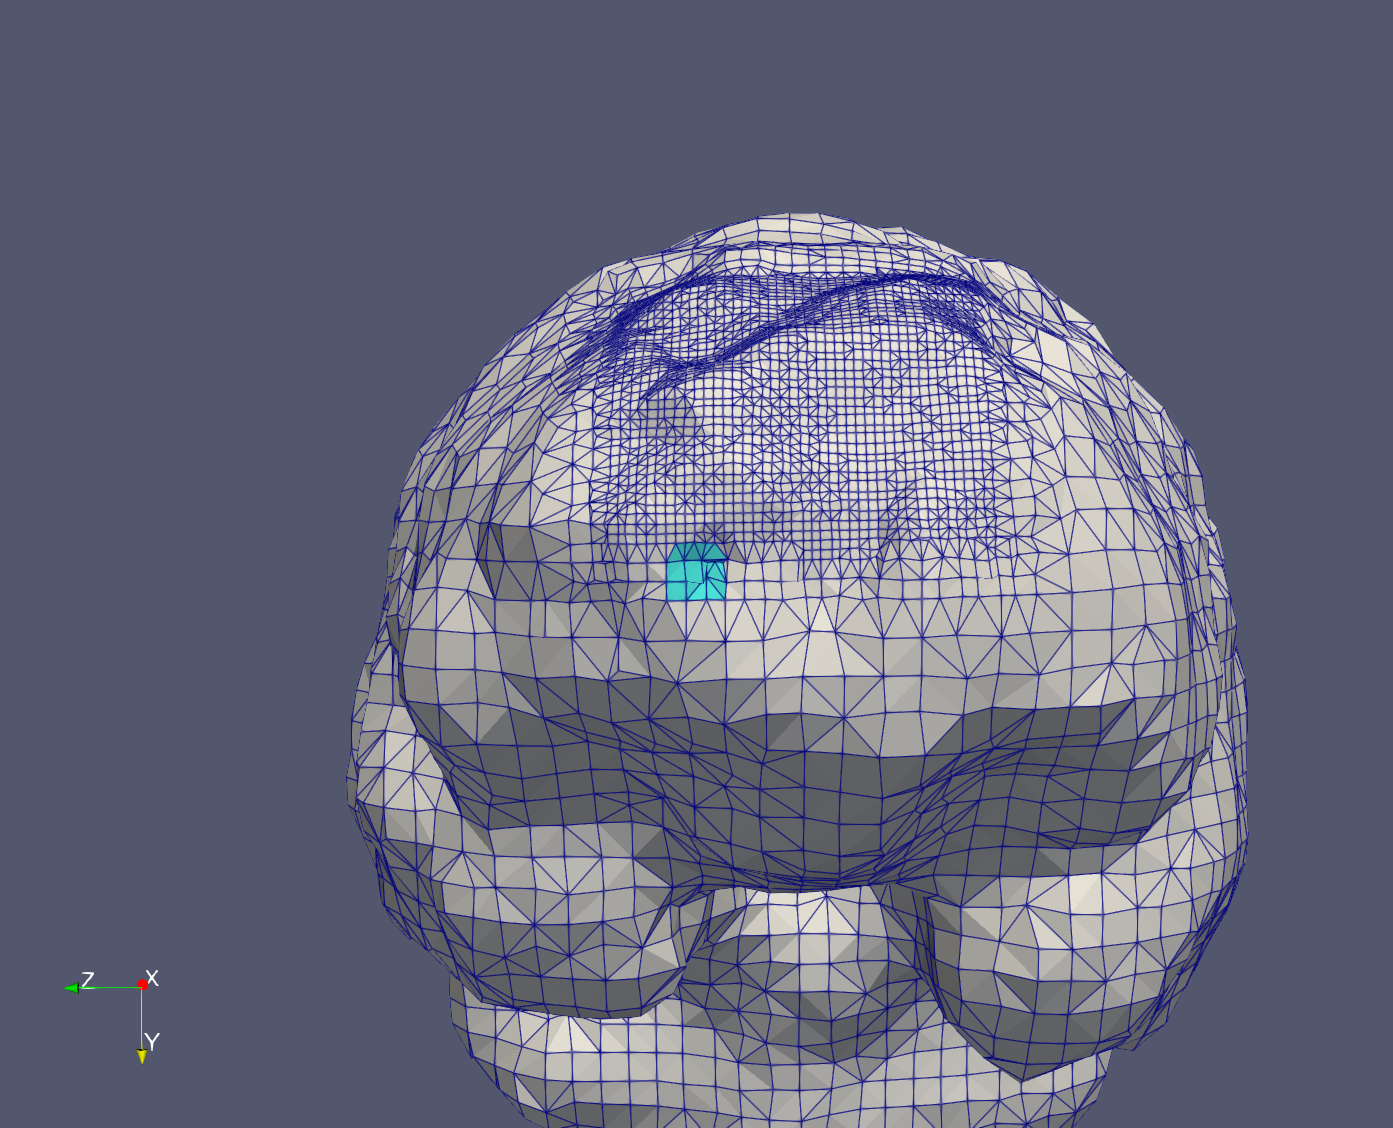
\includegraphics[width=1.0\textwidth]{figures/bad_quality_zone/zoom_out_bq_zone.png}
        \caption{Zoom out de sección extraída.}
    \end{subfigure}
    \begin{subfigure}[t]{0.45\textwidth}
        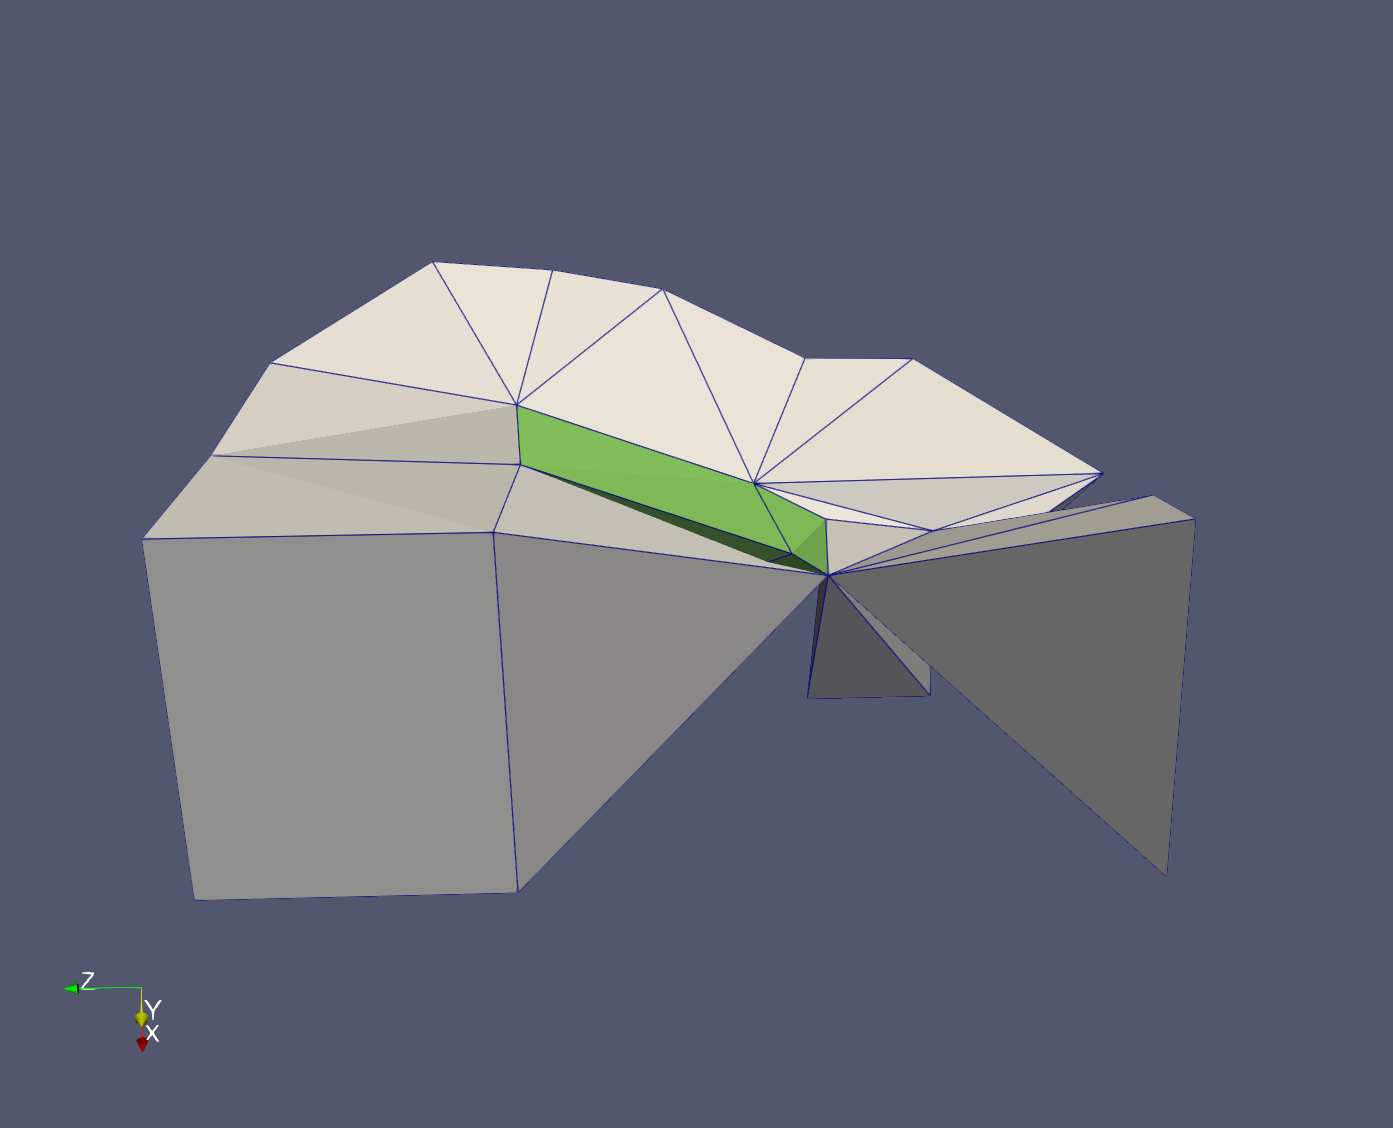
\includegraphics[width=1.0\textwidth]{figures/bad_quality_zone/bq_zone_02.png}
        \caption{Zona extraída con elementos de mala calidad resaltados.}
    \end{subfigure}
    \caption{ Zona a analizar para evidenciar elementos de mala calidad, esta zona se extrajo de la representación de la malla con un nivel 5 de refinamiento general y nivel 7 de refinamiento en la superficie entregada. En la imagen de la izquierda se muestra una visión general de la superficie de la malla demarcada por elementos con vértices azules y la zona a estudiar de color celeste. En la imagen de la derecha, la zona a estudiar y un par de elementos de mala calidad destacados con color verde. }
    Fuente: Elaboración propia.
    \label{fig:zoom_cortex_surf}
\end{figure}

% \begin{algorithm}
% \caption{Algoritmo para etiquetar elementos.}\label{alg:get_labeled_elements} 
% \SetKwInOut{KwIn}{Input}
% \SetKwInOut{KwOut}{Output}
% % functions
% \SetKwFunction{getLabeledElements}{GET\_LABELED\_ELEMENTS}
% \SetKwFunction{calculateJens}{CALCULATE\_JENS}
% \SetKwFunction{getOctant}{GET\_OCTANT}
% \SetKwFunction{getIndex}{GET\_INDEX}
% \SetKwFunction{getSubElementIndexes}{GET\_SUB\_ELEMENTS\_INDEXES}
% \SetKwFunction{add}{ADD}
% \SetKwFunction{size}{SIZE}
% % procedure
% \SetKwProg{myproc}{Procedure}{:}{}
% \KwIn{Malla Octree $M$, cota de calidad $T$.}
% \KwOut{Lista de Elementos de mala calidad etiquetados.}
% \myproc{\getLabeledElements{$M$, $T$}}
% {
%     $le$ \gets \, empty set \tcp*{Lista de Elementos etiquetados.} 
%     \For{ \textbf{each} $element$ \textbf{in} $M$} {
%         $q$ \gets \, \calculateJens{$element$}\;
%         \If{$q < T$} {
%             $element\_index$ \gets $element$.\getIndex{}\;
%             $le$.\add{$element\_index$}\;
%         }
%     }
%     \KwRet $lo$\;    
% }
% \end{algorithm}

\subsubsection{Análisis de la vecindad}

En esta sección de la malla, se puede observar a simple vista una superficie de naturaleza cóncava. Este tipo de geometría tiende a facilitar la aparición de elementos inválidos durante el proceso de generación de la malla.

Como se muestra en la \autoref{fig:zoom_cortex_surf_all}, los elementos inválidos son fácilmente identificables. Estos elementos, destacados en verde, crean áreas en la malla que no representan fielmente la geometría original y muestran incongruencias respecto a los elementos vecinos. En este contexto, los elementos inválidos generan una anomalía observable en relación a su entorno inmediato.

En particular, el par de elementos en verde está separado de los elementos adyacentes en su base. Esta separación indica una ruptura en la continuidad de la malla que no sigue la forma esperada de la superficie original. Este análisis resalta la importancia de prestar atención a la forma y las transiciones entre regiones de la malla para detectar y corregir estos problemas que pueden comprometer la calidad y precisión de la representación del modelo.

\begin{figure}[!ht]
    \centering
    \includegraphics[width=1.0\textwidth]{figures/bad_quality_zone/bq_zone_ALL.png}
    \caption{ Perspectivas de vecindario (gris) donde se encuentra un para de elementos inválidos (verde). }
    Fuente: Elaboración propia.
    \label{fig:zoom_cortex_surf_all}
\end{figure}


\subsection{Propuesta}

Para abordar y mejorar la calidad de los \elements{} inválidos en la malla, se propone refinar las localidades donde estos se encuentran. En términos específicos, esto implica realizar un refinamiento en los \octants{} que están asociados con los \elements{} inválidos.

% Entonces, en general, se necesitará luego de generar la malla, identificar y etiquetar los octantes que contengan elementos inválidos.  

% Luego, iterar nuevamente la malla para refinar aquellos octantes identificados y realizar las transformaciones pertinentes para mantener la congruencia en la malla.

% Realizar las iteraciones de los pasos anteriores las veces necesarias hasta obtener una malla congruente, sin elementos inválidos.

Se definirá el algoritmo de esta propuesta como el siguiente:

\begin{enumerate}
    \item Generación de malla inicial.
    
        La generación de la malla inicial, implica utilizar la herramienta \mesher{} para construir la malla inicial con las condiciones establecidas.
    \item Identificación y Etiquetado de Octantes.
        
        El etiquetador de \octants{}, una modificación del algoritmo presentado en \autoref{alg:get_labeled_octants} que permitirá persistir los \octants{} etiquetados.
    
    \item Refinamiento de Octantes Identificados.
        
        El refinamiento de una lista de \octants{} utilizando el parámetro `-l' del \mesher{}.
            
    \item Generación de estadísticas $J_{ENS}$.
    
   	 	Al finalizar la generación de la malla o refinamiento, se obtendrá y guardará de manera persistente su estadística para validar las condiciones de detención del algoritmo y generar un directorio historial con las mallas y sus correspondientes estadísticas para posterior análisis.
\end{enumerate}


Es importante, en este punto, mencionar que se escogió seleccionar la última malla generada como la ``malla solución'' porque el algoritmo se comporta de manera exponencial en la mayoría de los casos, comportamiento analizado en la \autoref{section:validation}.

\subsubsection{Generación de malla inicial.}


\begin{lstlisting}[style=Console,caption={Generador de malla, crea una malla refinada a nivel 5 y especificamente refina la superficie entregada a nivel 7, se exportará la malla con el nombre \textit{c\_5r7\_0}, en formato vtk y m3d.\\ Fuente: Elaboración propia.}]
input  >    ./mesher_roi -d ./data/cortex.mdl -s 5 -r ./data/cortex_surf_roi.mdl 7 -u c_5r7_0 -m -v
output >    All done in xxxx ms
\end{lstlisting}

% Para preparar esta malla inicial para su mejora, se realizó una modificación al algoritmo de \textit{MESHER\_GENERATOR}, permitiendo obtener, al finalizar la generación de la malla, estadísticas $J_{ENS}$ con la frecuencia de elementos, segunda columna en \autoref{code:jens_histo_c_5r7_0}, con $J_{ENS}$ menor a las cotas dispuestas en la primera columna.

% Esto se implementó exportando la información en un archivo con extensión '.histo', el histograma generado en \textit{JENS\_STADISTICS\_GENERATOR} y de esta manera, también lograr gestionar la información de forma óptima entre sistemas de información.

% Además, por defecto, \textit{MESHER\_GENERATOR} crea un archivo de respaldo con extensión '.oct' que guarda información de la malla, sus puntos y octantes definidos en la iteración.

%\breakpoint{06-08-2024}

Para mejorar la calidad de la malla inicial, se implementaron modificaciones específicas en el algoritmo \mesher{}. Estas modificaciones están diseñadas para evaluar y gestionar la calidad de los elementos generados, proporcionando estadísticas detalladas y facilitando la integración con otros sistemas de información.
Se ha actualizado el algoritmo \mesher{} para que, al finalizar la generación de la malla, se obtengan estadísticas de calidad $J_{ENS}$. Estas estadísticas se presentan en un formato que permite evaluar la calidad de los elementos en relación con ciertos umbrales predeterminados, además se modificó la información sobre los octantes que se guardan de manera persistente en el disco.

Puntos a destacar de esta implementación:
    
\begin{itemize}
    \item  Generación de Estadísticas $J_{ENS}$:

	Al finalizar la generación de la malla, el algoritmo calcula las estadísticas $J_{ENS}$, las cuales proporcionan una medida de la calidad de los \elements{}. Estas estadísticas se registran en cada iteración, creando un historial detallado que permite monitorear la calidad de la malla de manera continua.
	
	\item Exportación de datos en formato estándar:
	
	Para facilitar el análisis de estas estadísticas, los datos se almacenarán de forma persistente en un archivo con extensión \textit{.histo}. Este archivo contiene dos columnas clave: la primera registra los umbrales de calidad, mientras que la segunda muestra la frecuencia de elementos cuya calidad se encuentra por debajo de esos umbrales. Un ejemplo del contenido de este archivo se ilustra en la \autoref{code:jens_histo_c_5r7_0} , donde los intervalos de calidad están etiquetados con ``<intervalo\_fq\_bqe>'' para cada intervalo de calidad, y el nombre del archivo incluye un identificador de la iteración correspondiente.
	
	El archivo comienza con una cota que incluye los elementos con $J_{ENS}$ negativo, seguida de cotas progresivas, con excepciones en los primeros tres valores ($neg$, $0.03$, $0.05$), y luego con incrementos regulares de $0.05$. Esta disposición permite una evaluación sistemática de la calidad de los elementos a lo largo de un rango definido de valores $J_{ENS}$. Los intervalos y cotas superiores se mantuvieron consistentes con el formato de \jens{}, facilitando su integración con otros sistemas.
	
	El histograma generado por el módulo \jens{} es crucial, ya que proporciona una visualización clara y eficiente de la distribución de la calidad de los elementos dentro de la malla. Esto permite identificar rápidamente cómo se ven afectados los elementos en cada iteración, facilitando la toma de decisiones y el ajuste del refinamiento de la malla.
	    
		
		\begin{lstlisting}[style=TxtStyle,caption={Estructura de archivo con extensión \textit{.histo} que contiene un histograma con estadísticas de elementos $J_{ENS}$ de la malla de la iteración actual.\\ Fuente: Elaboración propia.},label={code:jens_histo_c_5r7_0}]
		____________________________________________
		 File: c_5r7_x.histo 
		____________________________________________
		negative <neg_fq_bqe>
		0.030000 <0.03_fq_bqe>
		0.050000 <0.05_fq_bqe>
		0.100000 <0.10_fq_bqe>
		0.150000 <0.15_fq_bqe>
		0.200000 <0.20_fq_bqe>
		0.250000 <0.25_fq_bqe>
		0.300000 <0.30_fq_bqe>
		0.350000 <0.35_fq_bqe>
		0.400000 <0.40_fq_bqe>
		0.450000 <0.45_fq_bqe>
		0.500000 <0.50_fq_bqe>
		0.550000 <0.55_fq_bqe>
		0.600000 <0.60_fq_bqe>
		0.650000 <0.65_fq_bqe>
		0.700000 <0.70_fq_bqe>
		0.750000 <0.75_fq_bqe>
		0.800000 <0.80_fq_bqe>
		0.850000 <0.85_fq_bqe>
		0.900000 <0.90_fq_bqe>
		0.950000 <0.95_fq_bqe>
		1.000000 <1.00_fq_bqe>
		\end{lstlisting}
		
	  \item Gestión de información entre sistemas:
		
	  La exportación en formato \textit{.histo} también permite una integración óptima de la información entre diferentes sistemas de procesamiento y análisis.
	  Esta gestión eficiente asegura que los datos de calidad de la malla sean accesibles y utilizables en otras aplicaciones o modificaciones al algoritmo en trabajos futuros, facilitando así el flujo de trabajo en entornos complejos de simulación o modelado.
	  
	  \item Respaldo de la información de la malla:
	  
	  Además de las estadísticas de calidad, se necesitará disponer de un estado de la malla, por defecto, \mesher{} crea un archivo de respaldo de extensión \textit{.oct}, que contiene una representación detallada de la malla, incluyendo la posición de los puntos y la definición de los octantes en cada iteración.
	  Este archivo es esencial para conservar un registro completo del estado de la malla en diferentes etapas del proceso de generación de la malla y su refinamiento.
		
	  Este archivo de respaldo, será modificado para incluir información adicional sobre los octantes, para posteriormente localizar correctamente octantes en base a sus identificadores únicos.
	  
	  Este archivo \textit{.oct} permite una fácil recuperación y revisión de la malla generada, facilitando la identificación de problemas y la evaluación de la calidad en etapas posteriores.
	  También sirve como un recurso valioso para la documentación y el seguimiento de los cambios realizados durante el proceso de refinamiento de la malla.
		\end{itemize}
    




% \begin{lstlisting}[style=TxtStyle,caption={Histograma con estádisticas de elementos Jens en malla inicial.\\ Fuente: Elaboración propia.},label={code:jens_histo_c_5r7_0}]
% ____________________________________________
%  File: c_5r7_0.oct 
% ____________________________________________
% <np> <ne> <no>

% <p_0_x> <p_0_y> <p_0_z>
% <p_1_x> <p_1_y> <p_1_z>
% <p_2_x> <p_2_y> <p_2_z>
% ...
% <p_NP-2_x> <p_NP-2_y> <p_NP-2_z>
% <p_NP-1_x> <p_NP-1_y> <p_NP-1_z>
% <p_NP_x> <p_NP_y> <p_NP_z>

% <octedpid_0_x> <octedpid_0_y> <ed_0_id>
% <octedpid_1_x> <octedpid_1_y> <ed_1_id>
% ...
% <octedpid_ED-1_x> <octedpid_ED-1_y> <ed_ED-1_id>
% <octedpid_ED_x> <octedpid_ED_y> <ed_ED_id>

% <npo_0> <pid_0_0> ... <pid_0_NPO_0> <rl_0> <octid_0>
% <nif_0> <if_0_0> ... <if_0_NIF_0>
% <npo_1> <pid_1_0> ... <pid_1_NPO_0> <rl_1> <octid_1>
% <nif_1> <if_1_0> ... <if_1_NIF_1>
% ...
% <npo_NO-1> <pid_NO-1_0> ... <pid_NO_NPO_0> <rl_NO> <octid_NO-1>
% <nif_NO-1> <if_NO-1_0> ... <if_NO-1_NIF_NO-1>
% <npo_NO> <pid_NO_0> ... <pid_NO_NPO_0> <rl_NO> <octid_NO>
% <nif_NO> <if_NO_0> ... <if_NO_NIF_NO-1>

% Geometric Transform
% <centroid_x> <centroid_y> <centroid_z>
% <coord_x> <coord_y> <coord_z>

% <octmeshid_0> <octmeshid_1>...<octmeshid_NO-1> <octmeshid_NO>
% \end{lstlisting}

% \begin{lstlisting}[style=TxtStyle,caption={Histograma con estádisticas de elementos Jens en malla inicial.\\ Fuente: Elaboración propia.},label={code:jens_histo_c_5r7_0}]
% ____________________________________________
%  File: c_5r7_0.oct 
% ____________________________________________
% 143105 598817 122438

% +2.85692000E-01  +2.21920000E-02  +1.91885460E+01
% +1.34949800E+02  +2.21920000E-02  +1.91885460E+01
% ...
% +1.37053927E+02  +9.04996396E+01  +6.33752064E+01
% +1.37053927E+02  +9.04996396E+01  +1.09665994E+02

% 0 1 21
% 0 3 22
% ...
% 142878 142879 0
% 142880 142881 0

% 8 37427 37436 37441 37439 22347 37431 37440 37434 7 34256
% 3 4491 4615 4723
% 8 37436 37428 37437 37441 37431 22339 37432 37440 7 34257
% 2 4615 4723
% ...
% 8 142881 142871 142868 142880 22312 22231 1134 22311 4 147370
% 0
% 8 142876 142881 142880 142875 22304 22312 22311 5201 4 147371
% 0

% Geometric Transform
% 0.000000 0.000000 0.000000
% 0.000000 0.000000 0.000000

% 0 0 1 ... 1 1 1 
% \end{lstlisting}

\subsubsection{Identificación y etiquetado de Octantes.}

Como se explicó en la sección de \textit{Análisis de la vecindad}, identificar y etiquetar los octantes se realizará por medio del algoritmo \ref{alg:get_labeled_octants}, adicional a esto, se creará un archivo con la extensión \textit{.ref} para persistir la información. Este archivo es crucial porque almacenará una lista detallada de los índices de los octantes que necesitan ser refinados. Es importante que esta lista sea persistente para, además de tener un historial de los octantes refinados en cada iteración, lograr convalidarlo con el trabajo existente en \mesher{}.

La persistencia de esta información permite rastrear los cambios realizados en cada iteración del refinamiento, asegurando una documentación completa y accesible del proceso. Facilita la revisión y análisis posterior pudiendo incluso, utilizar otros lenguajes de programación en el proceso.

\begin{lstlisting}[style=TxtStyle,caption={Lista de octantes a refinar en malla inicial.\\ Fuente: Elaboración propia.},label={code:oct_labeled_c_5r7_0}]
____________________________________________
 File: c_5r7_x.ref 
____________________________________________
<octid_0>
<octid_1>
...
<octid_NOL-1>
<octid_NOL>
\end{lstlisting}

En \autoref{code:oct_labeled_c_5r7_0}, se dispone un ejemplo del archivo \textit{.ref}, considerando $NOL$ la cantidad de octantes a refinar y $octid\_k$ los identificadores únicos de los octantes a refinar, siendo $k \in \{ 0, ..., NOL\}$.

\subsubsection{Refinamiento de Octantes Identificados.}

Teniendo en consideración la lista de octantes a refinar exportado en el archivo \textit{.ref}, queda entonces entregar esta lista a \mesher{}, junto con el listado debe entregarse también la malla de la iteración anterior.

De esta manera, en una posible iteración 3, por ejemplo, se utilizará el archivo \textit{.oct} y \textit{.ref} de la iteración 2, esto es comenzar con la malla generada en la iteración anterior como en \autoref{code:ref_oct_labeled_iter_3}, donde se definen los siguientes elementos:

\begin{itemize}
    \item \textit{-d ./data/cortex.mdl}: Corteza del cerebro a analizar. 
    \item \textit{-c c\_5r7\_2.oct}: Información sobre los octantes generados en la iteración anterior.
    \item \textit{-l ./c\_5r7\_2.ref}: Lista de Octantes a refinar.
    \item \textit{-t 0.0}: Treshold definido en cero.
    \item \textit{-u c\_5r7\_3}: Nombre base de los archivos a exportar en la iteración actual.
    \item \textit{-m}: Exportación en formato m3d.
    \item \textit{-v}: Exportación en formato vtk.
\end{itemize}

Lo anterior, refinará los Octantes de mala calidad de la malla en la iteración 2 según la cota definida en dicha iteración y analizará los nuevos elementos para definir una nueva lista de Octantes a refinar.
Esto se exportará con el nombre de la iteración actual, exportando los siguientes archivos.

\begin{itemize}
    \item \textit{c\_5r7\_3.oct}: Información sobre los puntos y octantes de la malla generada,
    \item \textit{c\_5r7\_3.ref}: Lista de Octantes a refinar en iteración actual.
    \item \textit{c\_5r7\_3.m3d}: Información sobre puntos, elementos y octantes de la malla generada para visualización en Geomview.
    \item \textit{c\_5r7\_3.vtk}: Información sobre puntos, elementos y octantes de la malla generada para visualización en Paraview.
\end{itemize}


\begin{lstlisting}[style=Console,caption={Generador de malla, crea una nueva malla, tomando como input la malla inicial \textit{c\_5r7\_0.oct}, la lista de octantes a refinar \textit{c\_5r7\_0.ref}, la cota de calidad $J_{ENS}$ definido en cero, se exportará la malla con el nombre \textit{c\_5r7\_1}, en formato vtk y m3d.\\ Fuente: Elaboración propia.},label={code:ref_oct_labeled_iter_3}]
input >     ./mesher_roi -d ./data/cortex.mdl -c ./c_5r7_2.oct -l ./c_5r7_2.ref -t 0.0 -u c_5r7_3 -m -v
output >    All done in xxxx ms
\end{lstlisting}


\subsubsection{Ciclo Iterativo de Evaluación y Refinamiento.}

Teniendo todo para generar un proceso iterativo, se propone entonces un algoritmo, \autoref{alg:propuesta_iter}, que ejecutará \mesher{} las veces necesarias hasta que ya no existan elementos de mala calidad.

Como se explicó en la Sección \ref{section:mesh_generator_definition}, \mesher{} tiene varias funcionalidades, para esta propuesta utilizaremos su funcionalidad de refinamiento general, que generará los refinamientos necesarios para las zonas definidas y definirá los elementos requeridos para consular la calidad de la malla.

Esta primera iteración será una ejecución de \mesher{}, donde se le entregará como input la malla principal a refinar que corresponde a los puntos que componen la corteza cerebral, también se le entregará la malla del área a refinar en la zona frontal de la corteza, su \textit{threshold} para la identificación de Octantes que contengan elementos de mala calidad y el nombre base para la exportación de los archivos.

El algoritmo además, propone una ejecución de \mesher{}} que se ejecutará en todas las iteraciones restantes, tomará la información de la malla generada en las iteraciones previas para refinar los Octantes identificados en de las iteraciones previas. Se le entregará como input la malla principal, los octantes y puntos definidos en la iteración anterior, la lista de Octantes a refinar en la iteración actual y que fueron identificados de la iteración previa, su \textit{threshold} y el nombre base para la exportación de los archivos. 

Por último, es necesario una condición de término del algoritmo, para ello se propone un evaluador de calidad denominado \textit{IMPROVER\_EVALUATOR}, este se ejecutará al final de cada iteración y consultará la existencia del archivo que contiene la lista de Octantes a refinar. 
Esto se realiza de esta manera, ya que, cuando no existe Octantes por refinar, es decir, no existen elementos de mala calidad, no se crea el archivo con extensión \textit{.ref}.

\begin{algorithm}
\caption{Algoritmo iterativo propuesto}\label{alg:propuesta_iter} 
\SetKwInOut{KwIn}{Input}
\SetKwInOut{KwOut}{Output}
% functions
\SetKwFunction{mesherGenerator}{mesher\_generator}
\SetKwFunction{improverEvaluator}{IMPROVER\_EVALUATOR}
\SetKwFunction{fileExist}{FILE\_EXIST}
\SetKwFunction{getFileLines}{GET\_FILE\_LINES}
\SetKwFunction{getFileLines}{GET\_FILE\_LINES}
% procedure
\SetKwProg{myproc}{Procedure}{:}{}
\KwIn{Malla corteza $main\_surf$.\\Superficie a refinar $ref\_surf$.\\ Nombre base para archivos de exportación $base\_name$.\\ Cota de calidad $T$.\\ Número máximo de iteraciones $I$.}
\KwOut{if successful,  volumetric mesh of \Omega that meet the $RLC$ with quality greather than $T$.}
\myproc{\generateMesh{$main\_surf$, $ref\_surf$, $base\_name$, $T$, $I$}}
{
    \ForEach{$i \in \{0, \dots, $I$\}$} {
        out\_name \gets\, base\_name + \_  + $i$ \;
        \If{$i == 0$} {
            \mesherGenerator(main\_surf, ref\_surf, threshold, out\_name) \;
        }
        \Else {
            prev\_iteration \gets \, $i-1$ \;
            base\_name\_prev \gets\, base\_name + \_  + prev\_iteration \;
            ref\_name\_prev \gets\, base\_name\_prev + .ref \;
            octs\_name\_prev \gets\, base\_name\_prev + .oct \;
            \mesherGenerator(main\_surf, octs\_name\_prev, ref\_name\_prev, threshold, out\_name) \;
        }
        \improverEvaluator{ref\_name\_prev, $i$} \;
    }
    $lo$ \gets \getFileLines{ref\_name\_prev} \;
    \textbf{PRINT} ``Finished, number of iterations exceeded.'' \;
    \textbf{PRINT} ``Octants to improve: $lo$'' \;
    \KwRet mesh\;    
}
\myproc{\improverEvaluator{$ref\_name$, $i$}}
{   
    \If{ \fileExist{ref\_name}} {
        $lo$ \gets \getFileLines{ref\_name} \;
        \textbf{PRINT} ``Octants to improve in iteration $i$: $lo$'' \;
    }
    \Else{
        \textbf{PRINT} ``No more Octants to improve in iteration $i$.'' \;
        \textbf{BREAK}\;
    }
}
\end{algorithm}



% Se debe desarrollar la solución propuesta. Los subcapítulos por poner aquí son propios del autor. Se sugiere mencionar metodología usada. Es conveniente incorporar figuras y tablas para aclarar la solución, que deben indicar el número de la figura, su nombre y su autor o fuente (si las diseñas tú, la fuente es ``Elaboración propia''). Ver ejemplos en esta página y en la siguiente.

% Cabe mencionar que aquí está la esencia del trabajo en lo que se refiere al aporte creativo del memorista, es el momento de demostrar que usted es un destacado profesional que creó, diseñó y/o llevó a cabo la solución propuesta.

% \subsection{EJEMPLO DE COMO CITAR FIGURAS E ILUSTRACIONES}

% Se colocó una imagen que se puede referenciar también desde el texto (Ver figura \ref{fig:malla}).

% \begin{figure}[h]
% \centering
% 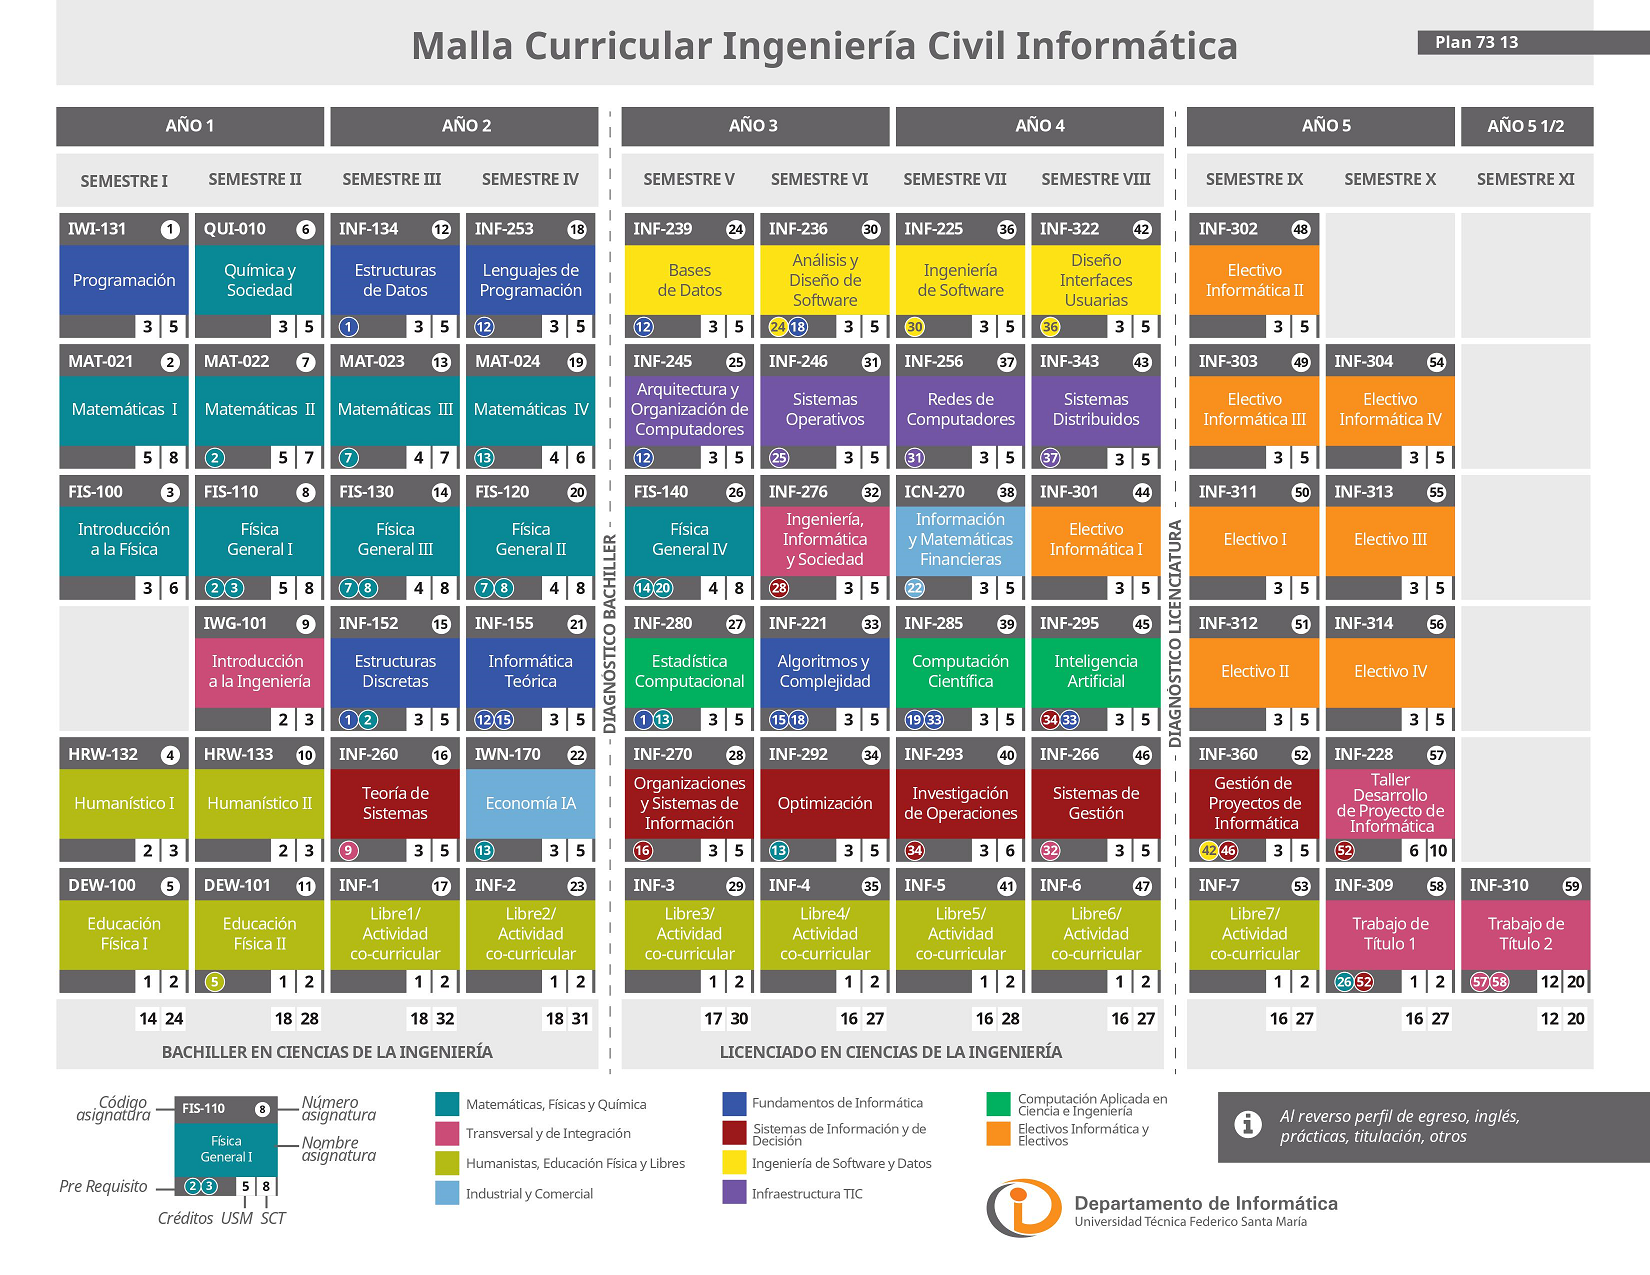
\includegraphics[width=0.8\textwidth]{malla_ingenieria_informatica}
% \caption{\label{fig:malla} Malla Curricular Ingeniería Civil Informática.} Fuente: Departamento de Informática.
% \end{figure}



% \begin{algorithm}
% \caption{Algoritmo de propuesta Donoso}\label{alg:propuesta_donoso} 
% \SetKwInOut{KwIn}{Input}
% \SetKwInOut{KwOut}{Output}
% % functions
% \SetKwFunction{generateMesh}{GENERATE\_MESH}
% \SetKwFunction{generateBalancedOctree}{GENERATE\_BALANCED\_OCTREE}
% \SetKwFunction{applyTransitionPatterns}{APPLY\_TRANSITION\_PATTERNS}
% \SetKwFunction{applySurfacePatterns}{APPLY\_SURFACE\_PATTERNS}
% \SetKwFunction{refineElement}{REFINE\_ELEMENT}
% \SetKwFunction{add}{ADD}
% \SetKwFunction{getBoundaryNodes}{GET\_BOUNDARY\_NODES}
% \SetKwFunction{getLabeledNodes}{GET\_LABELED\_NODES}
% % procedure
% \SetKwProg{myproc}{Procedure}{:}{}
% \KwIn{Refinement level constraints $RLC$, triangular surface mesh \Omega, quality threshold $T$, maximum number of iterations $I$.}
% \KwOut{if successful, volumetric mesh of \Omega that meet the $RLC$ with quality greather than $T$.}
% \myproc{\generateMesh{key, value}}
% {
%     $imesh$ \gets \generateBalancedOctree{RLC,\Omega}\;
%     $imesh$ \gets \applyTransitionPatterns{imesh}\;
%     $l$ \gets $empty set$ \;
%     \For{$1$ \textbf{to} $I$} {
%         $mesh$ \gets $imesh$ \;
%         $bnodes$ \gets \getBoundaryNodes{mesh, \Omega}\;
%         \For{ \textbf{each} $node$ \textbf{in} $bnodes$} {
%             \If{$node \in l$ \textbf{or} ($node$ is \textbf{inside} of \Omega \textbf{and} $node$ is \textbf{close} to \Omega)} {
%                 $node$.\refineElement{\Omega}\;
%             }
%         }
%         $mesh$ \gets \applySurfacePatterns{mesh}\;
%         $bnodes$ \gets \getBoundaryNodes{mesh, \Omega}\;
%         \For{\textbf{each} $node$ \textbf{in} $bnodes$} {
%             \If{$node$ is \textbf{outside} of \Omega} {
%                 $node$.\refineElement{\Omega}\;
%             }
%         }
%         $ln$ \gets \getLabeledNodes{mesh, $T$}\;
%         \If{$ln$ \textbf{is} empty}{
%             \KwRet mesh \;
%         }
%         \For{\textbf{each} $node$ in $ln$}{
%             $l$.\add(node)
%         }
%     }
%     \KwRet mesh\;    
% }
% \end{algorithm}


% \begin{algorithm}
% \caption{Algoritmo de propuesta Donoso}\label{alg:propuesta_donoso}
% \DontPrintSemicolon
% \SetKwInOut{KwIn}{Input}
% \SetKwInOut{KwOut}{Output}
% % functions
% \SetKwFunction{generateMesh}{GENERATE\_MESH}
% \SetKwFunction{refineOctant}{REFINE\_OCTANT}
% \SetKwFunction{generateBalancedOctree}{GENERATE\_BALANCED\_OCTREE}
% \SetKwFunction{applyTransitionPatterns}{APPLY\_TRANSITION\_PATTERNS}
% \SetKwFunction{applySurfacePatterns}{APPLY\_SURFACE\_PATTERNS}
% \SetKwFunction{refineOctant}{REFINE\_OCTANT}
% \SetKwFunction{add}{ADD}
% \SetKwFunction{getBoundaryNodes}{GET\_BOUNDARY\_NODES}
% \SetKwFunction{getLabeledOctants}{GET\_LABELED\_OCTANTS}
% \SetKwFunction{getRefinementLevel}{getRefinementLevel}
% % procedure
% \SetKwProg{myproc}{Procedure}{:}{}
% \KwIn{Restricciones de nivel de refinamiento $RLC$, malla de superficie triangular \Omega, umbral de calidad $T$, número máximo de iteraciones $I$.}
% \KwOut{Malla volumétrica de \Omega que cumpla con el $RLC$ con calidad superior a $T$.}
% \myproc{\generateMesh{key, value}}
% {
%     $imesh$ \gets \generateBalancedOctree{RLC,\Omega}\;
%     $imesh$ \gets \applyTransitionPatterns{imesh}\;
%     $l$ \gets empty set \tcp*{vector con octantes asociados a nodos de mala calidad.}
%     \For{$1$ \textbf{to} $I$} {
%         $mesh$ \gets $imesh$ \;
%         \tcc{Refinar octante asociado a nodo de mala calidad.}
%         \For{\textbf{each} $octant$ in $l$}{
%             $octant$.\refineOctant{\Omega}\;
%         }
%         \tcc{Obtener octantes con nodos de mala calidad.}
%         $lo$ \gets \getLabeledOctants{mesh, $T$}\;
%         \If{$lo$ \textbf{is} empty}{
%             \KwRet $mesh$ \;
%         }
%         \For{\textbf{each} $octant$ in $lo$}{
%             $l$.\add(octant)
%         }
%     }
%     \KwRet mesh\;    
% }
% \myproc{\refineOctant{\Omega}}
% {
%     $octant$ \gets this.octant \;
%     rl\_current \gets $octant$.\getRefinementLevel{} \;
    
% }
% \end{algorithm}


% \begin{algorithm}
% \SetKwInOut{KwIn}{Input}
% \SetKwInOut{KwOut}{Output}
% % functions
% \SetKwFunction{generateMesh}{GENERATE\_MESH}
% \SetKwFunction{generateBalancedOctree}{GENERATE\_BALANCED\_OCTREE}
% \SetKwFunction{applyTransitionPatterns}{APPLY\_TRANSITION\_PATTERNS}
% \SetKwFunction{applySurfacePatterns}{APPLY\_SURFACE\_PATTERNS}
% \SetKwFunction{projectOnto}{PROJECT\_ONTO}
% \SetKwFunction{add}{ADD}
% \SetKwFunction{getBoundaryNodes}{GET\_BOUNDARY\_NODES}
% % procedure
% \SetKwProg{myproc}{Procedure}{:}{}
% \KwIn{Refinement level constraints $RLC$, triangular surface mesh \Omega, quality threshold $T$, maximum number of iterations $I$.}
% \KwOut{if successful, volumetric mesh of \Omega that meet the $RLC$ with quality greather than $T$.}
% \myproc{\generateMesh{key, value}}
% {
%     $imesh$ \gets \generateBalancedOctree{RLC,\Omega}\;
%     $imesh$ \gets \applyTransitionPatterns{imesh}\;
%     $l$ \gets empty set \;
%     \For{$1$ \textbf{to} $I$} {
%         $mesh$ \gets $imesh$ \;
%         $bnodes$ \gets \getBoundaryNodes{mesh, \Omega}\;
%         \For{ \textbf{each} $node$ \textbf{in} $bnodes$} {
%             \If{$node \in l$ \textbf{or} ($node$ is \textbf{inside} of \Omega\, \& $node$ is \textbf{close} to \Omega)} {
%                 $node$.\projectOnto{\Omega} \;
%             }
%         }
%         $mesh$ \gets \applySurfacePatterns{mesh}\;
%         $bnodes$ \gets \getBoundaryNodes{mesh, \Omega}\;
%         \For{\textbf{each} $node$ \textbf{in} $bnodes$} {
%             \If{$node$ is \textbf{outside} of \Omega} {
%                 $node$.\projectOnto{\Omega} \;
%             }
%         }
%         \If{$ln$ \textbf{is} empty}{
%             \KwRet mesh \;
%         }
%         \For{\textbf{each} $node$ in $ln$}{
%             $l$.\add(node)
%         }
%     }
    
%     \KwRet null\;    
% }
% \caption{Algoritmo de propuesta Daines \\ Fuente: \cite{daines2018repairing}}
% \label{alg:propuesta_daines} 
% \end{algorithm}





% \begin{algorithm}
% \SetKwInOut{KwIn}{Input}
% \SetKwInOut{KwOut}{Output}
% % functions
% \SetKwFunction{main}{MAIN}
% \SetKwFunction{getInput}{GET\_INPUT}
% \SetKwFunction{generateMesh}{GENERATE\_MESH}
% \SetKwFunction{exportMesh}{EXPORT\_MESH}
% \SetKwFunction{saveData}{SAVE\_DATA}
% \SetKwFunction{generateBalancedOctree}{GENERATE\_BALANCED\_OCTREE}
% \SetKwFunction{applyTransitionPatterns}{APPLY\_TRANSITION\_PATTERNS}
% \SetKwFunction{applySurfacePatterns}{APPLY\_SURFACE\_PATTERNS}
% \SetKwFunction{projectOnto}{PROJECT\_ONTO}
% \SetKwFunction{add}{ADD}
% \SetKwFunction{getBoundaryNodes}{GET\_BOUNDARY\_NODES}
% % procedure
% \SetKwProg{myproc}{Procedure}{:}{}
% \KwIn{Refinement level constraints $RLC$, triangular surface mesh \Omega.}
% \KwOut{Volumetric mesh of \Omega that meets $RLC$.}
% \myproc{\main{argc}}
% {
%     $inputs$ \gets \getInput{argc}\;
%     $mesh$  \gets \generateMesh{inputs}\;
%     \exportMesh{mesh}\;
% }
% \caption{Algoritmo de generación de mallas Octree con elementos mixtos y varios niveles de refinamiento.\\ Fuente: \cite{daines2018repairing}}
% \label{alg:propuesta_daines} 
% \end{algorithm}
\newpage
\secnumbersection{Validación de la solución}


% Se debe validar la solución propuesta. Esto significa probar o demostrar que la solución propuesta es válida para el entorno donde fue planteada.

% Tradicionalmente es una etapa crítica, pues debe comprobarse por algún medio que vuestra propuesta es básicamente válida. En el caso de un desarrollo de software es la construcción y sus pruebas; en el caso de propuestas de modelos, guías o metodologías podrían ser desde la aplicación a un caso real hasta encuestas o entrevistas con especialistas; en el caso de mejoras de procesos u optimizaciones, podría ser comparar la situación actual (previa a la memoria) con la situación final (cuando la memoria está ya implementada) en base a un conjunto cuantitativo de indicadores o criterios.

% \subsection{EJEMPLO DE COMO CITAR TABLAS}

% Se colocó una tabla que se puede referenciar también desde el texto (Ver tabla \ref{table:coloquios}).

% \begin{table}[h]
%     \centering
%     \caption{\label{table:coloquios} Coloquios del Ciclo de Charlas Informática.} Fuente: Elaboración Propia.
%     \begin{tabular}{|p{7cm}|p{7cm}|}
%         \hline
%         Título Coloquio & Presentador, País \\
%         \hline
%         ``Sensible, invisible, sometimes tolerant, heterogeneous, decentralized and interoperable... and we still need to assure its quality...''' & Guilherme Horta Travassos, Brasil.\\
%         \hline
%         ``Dispersed Multiphase Flow Modeling: From Environmental to Industrial Applications''' & Orlando Ayala, EE.UU.\\
%         \hline
%         ``Líneas de Producto Software Dinámicas para Sistemas atentos el Contexto''' & Rafael Capilla, España.\\
%         \hline
%         ... & ... \\
%         \hline
%     \end{tabular}
% \end{table}

% \subsection{Implementación}

\subsection{Stack de tecnologías}

En primera instancia existe la tentación por implementar una modificación completa de la herramienta \textit{MESHER\_GENERATOR}, esto es viable pero se descarta cuando se prioriza la escalabilidad y mantenibilidad de código. Sobre la eficiencia y rapidez de la propuesta, que son características importantes que evidencian calidad, se evaluarán en secciones posteriores.
En \textit{MESHER\_GENERATOR} sólo se realizarán las modificaciones descritas en las secciones anteriores que incluyen funcionalidades para identificar y exportar los Octantes a refinar, para generar estadísticas al finalizar el refinamiento en las mallas y las pequeñas modificaciones a las funcionalidades de exportación de la información de los Octantes para luego identificarlos globalmente y así refinar los Octantes correctos.

Entonces, como debemos ejecutar \textit{MESHER\_GENERATOR}, existen varias formas de realizar esto, pero se escogerá la que utilice menos recursos para ejecutar llamadas a sistema como lo hace \textit{bash} en linux. Ya que se requiere de funcionalidades básicas como iteraciones y manipulación de archivos, esta es una buena herramienta a utilizar.

\subsection{Proceso de análisis}

Para validar la propuesta, se utilizará una serie de mallas con diferentes complejidades.
\begin{itemize}
    \item Malla de corteza cerebral con área de refinamiento prismática en la zona frontal.

        Propuesta inicial, de por sí la malla de corteza cerebral posee una complejidad media, contiene algunas zonas cóncavas que podrían complejizar el refinamiento. El prisma se posicionará en la zona del lóbulo frontal.
    \item Malla de corteza cerebral con área de refinamiento prismática en la zona trasera.

        En la zona trasera, lóbulo occipital de la corteza cerebral, de naturaleza cóncava e irregular se posicionará el prisma para refinar localmente, esto con el fin de complejizar el trabajo del algoritmo.
    \item Malla de Moai con área de refinamiento prismática en la zona superior.

        Para este análisis se escogió una representación de un Moai, que naturalmente no posee múltiples zonas cóncavas, entonces se aplicará el área de refinamiento en la zona superior donde se presenta la mayor cantidad de zonas cóncavas. 
    \item Malla de Moai con área de refinamiento prismática en la zona inferior.

        Se utilizará también la zona inferior, que no posee mayor nivel de complejidad respecto a su concavidad, con motivo de aumentar el universo de soluciones.
    \item Malla de paladar con área de refinamiento prismática en la zona superior.

        Esta representación posee áreas muy finas con respecto a el resto de la malla, entonces se aplicó un área de refinamiento adicional en la zona superior por su complejidad en función de concavidad.
    \item Malla de coxis.

        En general esta representación es muy compleja, presenta zonas muy pequeñas y con múltiples concavidades.
\end{itemize}

A cada una de estas mallas se les aplicará el algoritmo propuesto con un threshold cero y cien iteraciones como cota superior. 
Luego de iterar las mallas, se analizará sus estadísticas sobre Elementos de mala calidad.

\subsection{Ejecución}

En cada malla dependiendo de su complejidad se aplicará o no, un área prismática para refinar localmente, de esta manera añadir consistencia a los resultados.

La única malla a la que no se le aplicará el área prismática es la malla de coxis debido a su compleja naturaleza explicada en la sección anterior.

\subsubsection{Malla de corteza cerebral}

Al implementar el algoritmo propuesto en la malla de corteza cerebral, entregándole como input el threshold definido en esta propuesta, el modelo de la corteza, el modelo de la superficie prismática a refinar, la base de nombre de los archivos exportados y una cota de cien iteraciones.  Obtenemos el siguiente output \ref{out:cortex_1}, que nos muestra un identificador de cada iteración con la cantidad de Octantes a refinar al finalizar dicha iteración, finalizando exitosamente en la cuarta iteración con una malla sin elementos inválidos y reduciendo la cantidad de Octantes a refinar casi de manera exponencial.

Luego se ejecutó el algoritmo con la zona a refinar en el lóbulo occipital con el siguiente output \ref{out:cortex_2}.

Si bien, en esta ocasión se logró obtener una malla válida con algunas iteraciones adicionales, la cantidad de Elementos inválidos se comporta similar a el caso anterior.


\begin{lstlisting}[style=Console,caption={Output de ejecución algoritmo propuesto en malla de corteza cerebral con zona a refinar en lóbulo frontal.\\ Fuente: Elaboración propia.},label={out:cortex_1}]
input  >    ./script.sh 0.0 ./data/cortex.mdl ./data/cortex_surf_roi.mdl c_5r7 100
output >    Threshold: 0.0
            Main surface: ./data/cortex.mdl
            Reference surface: ./data/cortex_surf_roi.mdl
            Base name: c_5r7
            Number of iterations: 100
            Octants to improve in iteration 0: 21
            Octants to improve in iteration 1: 7
            Octants to improve in iteration 2: 2
            Octants to improve in iteration 3: 1
            No more Octants to improve in iteration 4.
\end{lstlisting}

\begin{lstlisting}[style=Console,caption={Output de ejecución algoritmo propuesto en malla de corteza cerebral con zona a refinar en lóbulo occipital.\\ Fuente: Elaboración propia.},label={out:cortex_2}]
input  >    ./script.sh 0.0 ./data/cortex.mdl ./data/cortex_surf_roi_2.mdl c_5r7_2 100
output >    Threshold: 0.0
            Main surface: ./data/cortex.mdl
            Reference surface: ./data/cortex_surf_roi_2.mdl
            Base name: c_5r7_2
            Number of iterations: 100
            Octants to improve in iteration 0: 52
            Octants to improve in iteration 1: 27
            Octants to improve in iteration 2: 11
            Octants to improve in iteration 3: 6
            Octants to improve in iteration 4: 7
            Octants to improve in iteration 5: 3
            No more Octants to improve in iteration 6.
\end{lstlisting}

\begin{figure}[!ht]
    \centering
    \begin{subfigure}[t]{0.45\textwidth}
        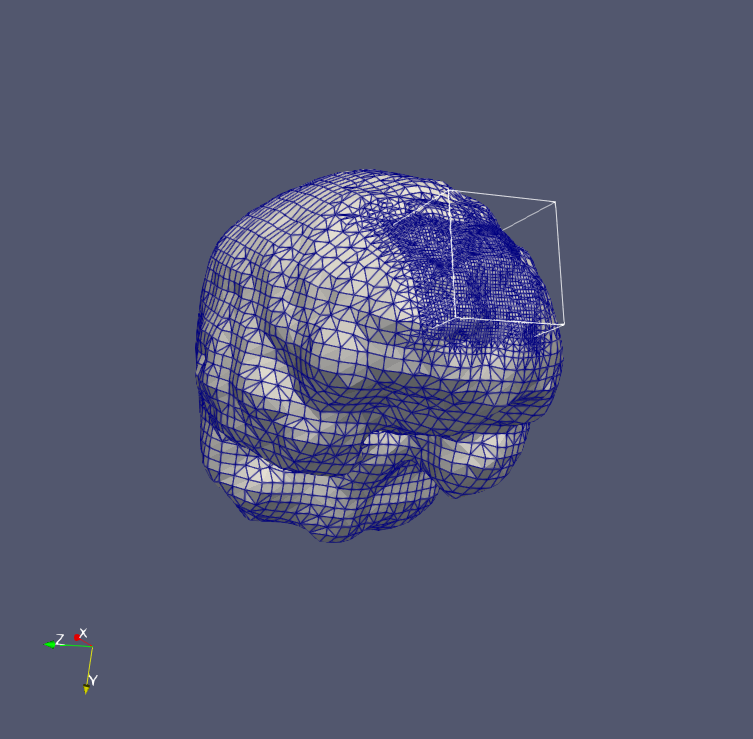
\includegraphics[width=1.0\textwidth]{figures/meshes/c_5r7_01.png}
        \caption{Representación corteza cerebral con refinamiento en lóbulo frontal.}
    \end{subfigure}
    \begin{subfigure}[t]{0.45\textwidth}
        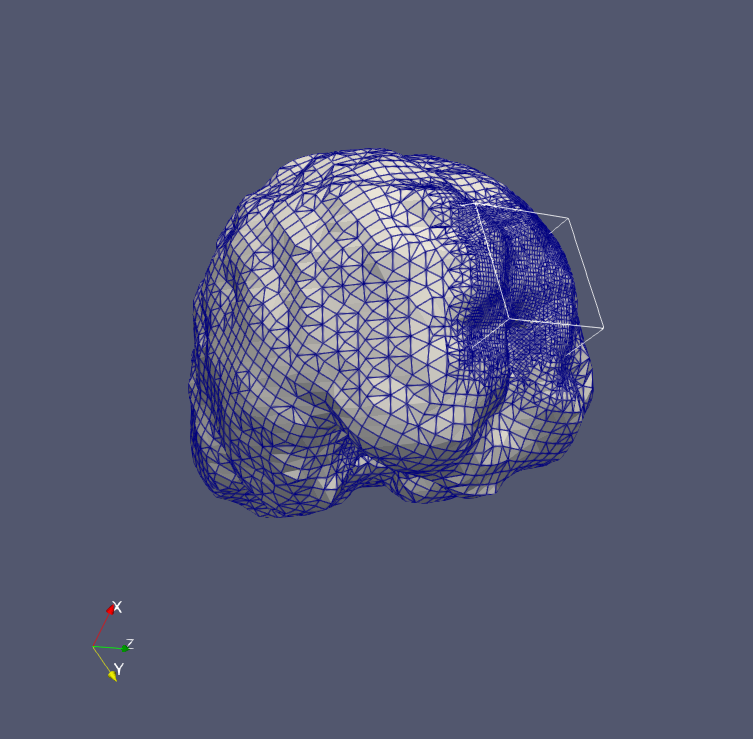
\includegraphics[width=1.0\textwidth]{figures/meshes/c_5r7_2_01.png}
        \caption{Representación corteza cerebral con refinamiento en lóbulo occipital.}
    \end{subfigure}
    \caption{ Diferentes localidades de refinamiento en corteza cerebral. }
    Fuente: Elaboración propia.
    \label{fig:c_5r7_all}
\end{figure}


\subsubsection{Malla de Moai}

La ejecución del algoritmo en la malla de Moai para los casos con refinamiento inferior y superior, como podemos ver en \autoref{out:moai_1} y \autoref{out:moai_2}, respectivamente. En ambos casos se logró una malla válida en aproximadamente 5 iteraciones, pero a diferencia de los casos anteriores, como la corteza cerebral y la zona inferior en el Moai, la malla de Moai en la zona superior, se comporta aumentando en un grado menor la cantidad de Octantes por refinar entre la primera y segunda iteración, luego disminuye la cantidad de Octantes manteniendo el aparente modelo exponencial.

\begin{lstlisting}[style=Console,caption={Output de ejecución algoritmo propuesto en malla de Moai con zona a refinar en zona inferior.\\ Fuente: Elaboración propia.},label={out:moai_1},float,floatplacement=H]
input  >    ./script.sh 0.0 ./data/moai.mdl ./data/moai_surf_roi.mdl moai_5r7 100
output >    Threshold: 0.0
            Main surface: ./data/moai.mdl
            Reference surface: ./data/moai_surf_roi.mdl
            Base name: moai_5r7
            Octants to improve in iteration 0: 22
            Octants to improve in iteration 1: 5
            Octants to improve in iteration 2: 2
            Octants to improve in iteration 3: 1
            Octants to improve in iteration 4: 1
            No more Octants to improve in iteration 5.
\end{lstlisting}


\begin{lstlisting}[style=Console,caption={Output de ejecución algoritmo propuesto en malla de Moai con zona a refinar en zona superior.\\ Fuente: Elaboración propia.},label={out:moai_2}, float,floatplacement=H]
input  >    ./script.sh 0.0 ./data/moai.mdl ./data/moai_surf_roi_2.mdl moai_5r7_2 100
output >    Threshold: 0.0
            Main surface: ./data/moai.mdl
            Reference surface: ./data/moai_surf_roi_2.mdl
            Base name: moai_5r7_2
            Number of iterations: 100
            Octants to improve in iteration 0: 10
            Octants to improve in iteration 1: 12
            Octants to improve in iteration 2: 9
            Octants to improve in iteration 3: 3
            No more Octants to improve in iteration 4.
\end{lstlisting}


\begin{figure}[!ht]
    \centering
    \begin{subfigure}[t]{0.45\textwidth}
        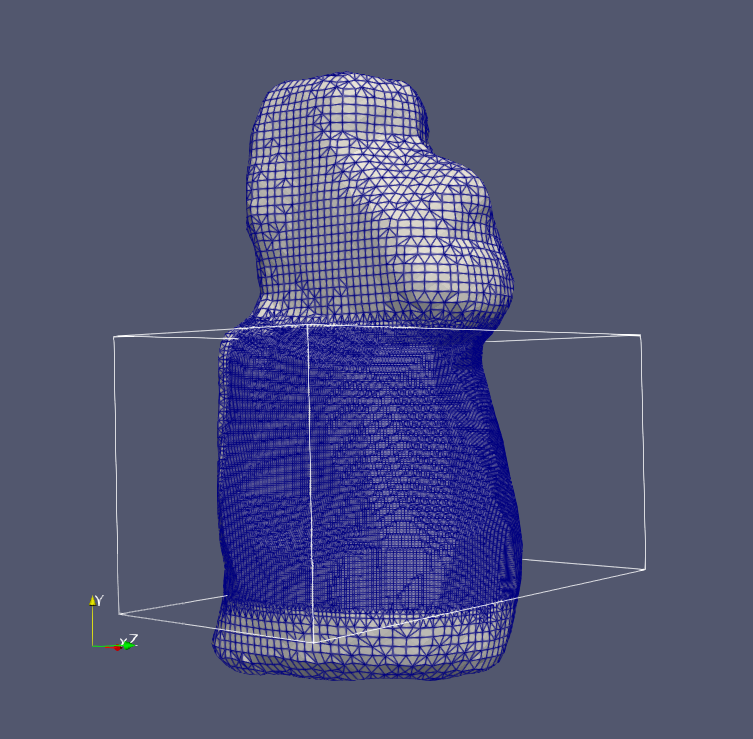
\includegraphics[width=1.0\textwidth]{figures/meshes/moai_5r7_01.png}
        \caption{Representación Moai con refinamiento en zona inferior.}
    \end{subfigure}
    \begin{subfigure}[t]{0.45\textwidth}
        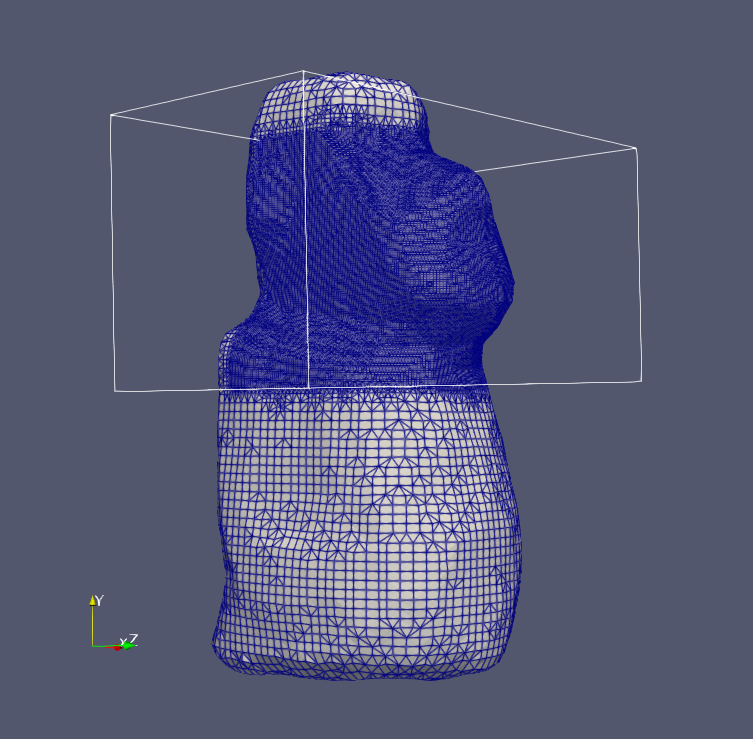
\includegraphics[width=1.0\textwidth]{figures/meshes/moai_5r7_2_01.png}
        \caption{ Representación Moai con refinamiento en zona superior. }
    \end{subfigure}
    \caption{ Diferentes localidades de refinamiento en Moai. }
    Fuente: Elaboración propia.
    \label{fig:moai_5r7_all}
\end{figure}

\subsubsection{Malla de paladar}


\begin{lstlisting}[style=Console,caption={Output de ejecución algoritmo propuesto en malla de Moai con zona a refinar en zona superior.\\ Fuente: Elaboración propia.},label={out:palate_1}, float,floatplacement=H]
input  >    ./script.sh 0.0 ./data/palate.mdl ./data/palate_surf_roi.mdl palate_5r7 100
output >    Threshold: 0.0
            Main surface: ./data/palate.mdl
            Reference surface: ./data/palate_surf_roi.mdl
            Base name: palate_5r7
            Number of iterations: 100
            Octants to improve in iteration 0: 33
            Octants to improve in iteration 1: 17
            Octants to improve in iteration 2: 6
            Octants to improve in iteration 3: 1
            Octants to improve in iteration 4: 1
            No more Octants to improve in iteration 5.
\end{lstlisting}



En el caso de la malla de paladar, podemos 

\begin{figure}[!ht]
    \centering
    \begin{subfigure}[t]{0.8\textwidth}
        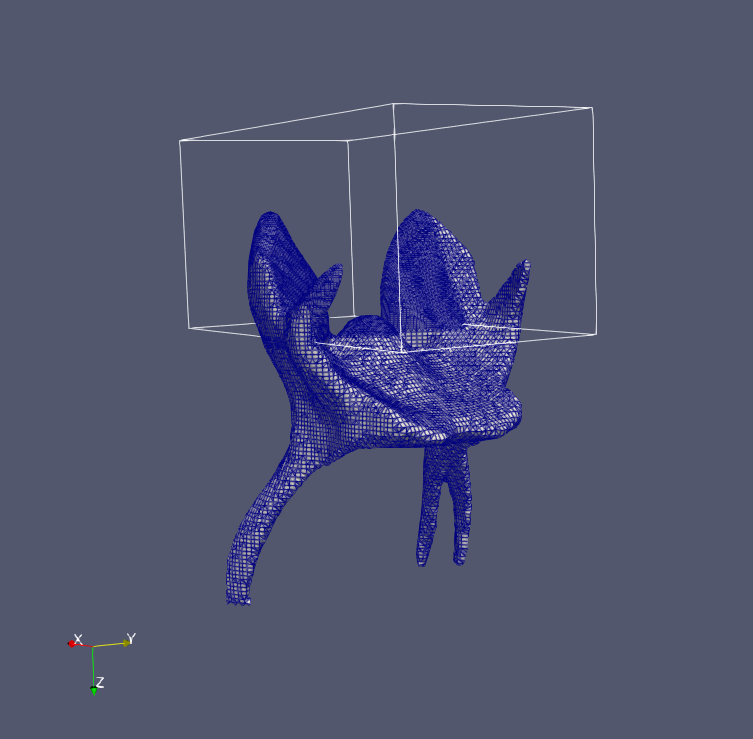
\includegraphics[width=1.0\textwidth]{figures/meshes/palate_5r7_01.png}
        % \caption{Representación Paladar con refinamiento en zona superior.}
    \end{subfigure}
    \caption{ Representación Paladar con refinamiento en zona superior. }
    Fuente: Elaboración propia.
    \label{fig:palate_5r7_all}
\end{figure}

\subsubsection{Malla de coxis}


\begin{lstlisting}[style=Console,caption={Output de ejecución algoritmo propuesto en malla de Moai con zona a refinar en zona superior.\\ Fuente: Elaboración propia.},label={out:moai_2}, float,floatplacement=H]
input  >    ./script.sh 0.0 ./data/palate.mdl ./data/palate_surf_roi.mdl palate_5r7 100
output >    Threshold: 0.0
            Main surface: ./data/palate.mdl
            Reference surface: ./data/palate_surf_roi.mdl
            Base name: palate_5r7
            Number of iterations: 100
            Octants to improve in iteration 0: 33
            Octants to improve in iteration 1: 17
            Octants to improve in iteration 2: 6
            Octants to improve in iteration 3: 1
            Octants to improve in iteration 4: 1
            No more Octants to improve in iteration 5.
\end{lstlisting}




\begin{figure}[!ht]
    \centering
    \begin{subfigure}[t]{0.8\textwidth}
        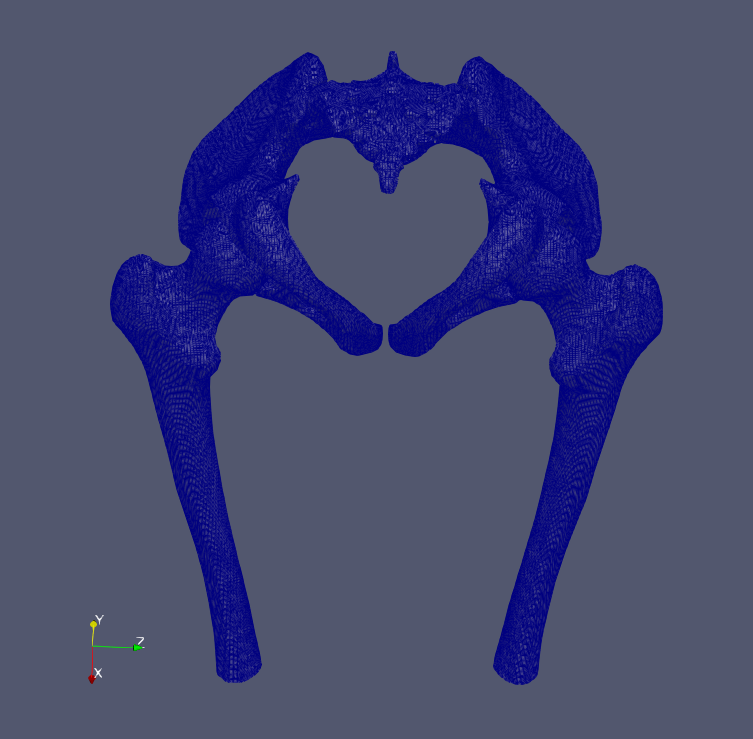
\includegraphics[width=1.0\textwidth]{figures/meshes/coxis_8r9_01.png}
    \end{subfigure}
    \caption{ Representación Coxis sin refinamiento local. }
    Fuente: Elaboración propia.
    \label{fig:coxis_8r9_all}
\end{figure}



\subsection{Análisis de los resultados}

\subsubsection{Análisis de la tasa de reducción de la cantidad de Octantes por refinar en cada iteración }

\begin{itemize}
    \item Definición de una secuencia exponencial.

    Para determinar si la secuencia de números $27, 7, 2, 1$ se reduce de manera exponencial, es esencial revisar cómo se comportan las reducciones entre cada par de números consecutivos y si sigue un patrón consistente con la reducción exponencial.

    Una reducción exponencial sigue la forma:
    $$y = a \cdot r^n$$
     
    donde:
    
    \begin{itemize}
        \item y es el valor en la n-ésima posición.
        \item a es el valor inicial (en nuestro caso, 21).
        \item r es la razón de reducción (un valor menor a 1).
        \item n es la posición en la secuencia.
    \end{itemize}
    
    Para verificar si una secuencia sigue una reducción exponencial, podemos examinar si el cociente entre cada par de términos consecutivos es aproximadamente constante. Es decir, si $\frac{y_{n+1}}{y_n}$ es constante.

    \item Cálculo del cociente entre términos consecutivos

    Calculamos el cociente entre cada par de números consecutivos en la secuencia:

    \begin{itemize}
        \item  Entre 21 y 7: $\frac{7}{21} \approx 0.333$
        \item  Entre 7 y 2: $\frac{2}{7} \approx 0.286$
        \item  Entre 2 y 1: $\frac{1}{2} = 0.5$
    \end{itemize}

    \item Evaluación de los Cocientes.

    Para una reducción exponencial pura, los cocientes entre términos consecutivos deberían ser aproximadamente iguales. En este caso, los valores no son iguales, pero están en un rango que sugiere una tendencia decreciente. Sin embargo, la variabilidad entre los cocientes sugiere que la secuencia no se reduce de manera perfectamente exponencial con una sola razón común.

    \item Ajuste a un modelo exponencial

    Podemos intentar ajustar un modelo exponencial para ver si se adapta razonablemente a los datos:
    Si consideramos $a  = 21$(valor inicial), podemos buscar una razón $r$ que mejor ajuste la reducción de la secuencia.
    
    Para esto, podemos resolver la ecuación $$y = 21 \cdot r^n$$ para cada $n$ y encontrar el $r$ promedio que mejor describa la secuencia. Aunque los cocientes no son constantes, podemos ver si hay un $r$ promedio que se ajuste razonablemente.

    \item Cálculo promedio geométrico

    El promedio geométrico de los cocientes es una manera de obtener una aproximación de la razón $r$:

        $$ r \approx \sqrt[3]{ \left( \frac{7}{21} \times \frac{2}{7} \times \frac{1}{2} \right) }$$

    Calculamos el valor:

    $$ r \approx \sqrt[3]{0.333 \times 0.286 \times 0.5 \approx 0.36} $$

    Este $r$ promedio indica que la secuencia puede aproximarse por una reducción exponencial con una razón cercana a $0.36$.

    Gráficamente podemos ver el ajuste del comportamiento de la cantidad de Octantes por refinar en cada iteración y los datos reales en \autoref{fig:exponential_fit}. Si bien este ajuste funciona muy bien para este caso, no podemos concluir que este algoritmo funcionará de esta manera para otros casos.

    % \begin{figure}[!ht]
    % \centering
    % \includegraphics[width=1.0\textwidth]{figures/analysis/exponential_fit.png}
    % \caption{ Ajuste exponencial de la cantidad de Octantes por refinar en cada iteración sobre los valores reales.\\  Fuente: Elaboración propia.}
    % \label{fig:exponential_fit}
    % \end{figure}
\end{itemize}

\subsection{Resultados}

Para analizar el comportamiento del algoritmo, nos enfocaremos en ajustar la cantidad de iteraciones a algún modelo conocido, entregar una hipótesis sobre la anomalía en la malla del coxis, comparar con los resultados entregados en \cite{daines2018repairing}.

\subsubsection{Ajuste de la cantidad de iteraciones}

El algoritmo propuesto se comporta de muy buena manera para todas las mallas a excepción de la malla que representa el coxis, cuando logra converger a una malla válida, es posible reducir considerablemente la cantidad de Octantes por refinar en muy pocas iteraciones, a simple vista se podría entregar una hipótesis sobre el comportamiento de la reducción en la cantidad de Octantes por refinar en cada iteración.

Para esto, se construyó la siguiente tabla con el número de Octantes por refinar en cada iteración para las diferentes mallas, \autoref{table:num_octs_ref}.



\begin{table}[!ht]
\begin{tabular}{|lllllll|}
\hline
\multicolumn{7}{|c|}{Número de Octantes por refinar en cada iteración}                                                                                                                                                                                                                     \\ \hline
\multicolumn{1}{|l|}{\textbf{N° Iteración}} & \multicolumn{1}{l|}{\textbf{cortex\_5r7}} & \multicolumn{1}{l|}{\textbf{cortex\_5r7\_2}} & \multicolumn{1}{l|}{\textbf{moai\_5r7}} & \multicolumn{1}{l|}{\textbf{moai\_5r7}} & \multicolumn{1}{l|}{\textbf{palate\_6r7}} & \textbf{coxis\_7} \\ \hline
\multicolumn{1}{|l|}{1}                     & \multicolumn{1}{l|}{21}                   & \multicolumn{1}{l|}{52}                      & \multicolumn{1}{l|}{22}                 & \multicolumn{1}{l|}{10}                 & \multicolumn{1}{l|}{33}                   & 211               \\ \hline
\multicolumn{1}{|l|}{2}                     & \multicolumn{1}{l|}{7}                    & \multicolumn{1}{l|}{27}                      & \multicolumn{1}{l|}{5}                  & \multicolumn{1}{l|}{12}                 & \multicolumn{1}{l|}{17}                   & 488               \\ \hline
\multicolumn{1}{|l|}{3}                     & \multicolumn{1}{l|}{2}                    & \multicolumn{1}{l|}{11}                      & \multicolumn{1}{l|}{2}                  & \multicolumn{1}{l|}{9}                  & \multicolumn{1}{l|}{6}                    & 341               \\ \hline
\multicolumn{1}{|l|}{4}                     & \multicolumn{1}{l|}{1}                    & \multicolumn{1}{l|}{6}                       & \multicolumn{1}{l|}{1}                  & \multicolumn{1}{l|}{3}                  & \multicolumn{1}{l|}{1}                    & 463               \\ \hline
\multicolumn{1}{|l|}{5}                     & \multicolumn{1}{l|}{0}                    & \multicolumn{1}{l|}{7}                       & \multicolumn{1}{l|}{1}                  & \multicolumn{1}{l|}{0}                  & \multicolumn{1}{l|}{1}                    & 528               \\ \hline
\multicolumn{1}{|l|}{6}                     & \multicolumn{1}{l|}{}                     & \multicolumn{1}{l|}{3}                       & \multicolumn{1}{l|}{0}                  & \multicolumn{1}{l|}{}                   & \multicolumn{1}{l|}{0}                    & 567               \\ \hline
\multicolumn{1}{|l|}{7}                     & \multicolumn{1}{l|}{}                     & \multicolumn{1}{l|}{0}                       & \multicolumn{1}{l|}{}                   & \multicolumn{1}{l|}{}                   & \multicolumn{1}{l|}{}                     & 665               \\ \hline
\multicolumn{1}{|l|}{8}                     & \multicolumn{1}{l|}{}                     & \multicolumn{1}{l|}{}                        & \multicolumn{1}{l|}{}                   & \multicolumn{1}{l|}{}                   & \multicolumn{1}{l|}{}                     & 767               \\ \hline
\multicolumn{1}{|l|}{9}                     & \multicolumn{1}{l|}{}                     & \multicolumn{1}{l|}{}                        & \multicolumn{1}{l|}{}                   & \multicolumn{1}{l|}{}                   & \multicolumn{1}{l|}{}                     & 887               \\ \hline
\multicolumn{1}{|l|}{10}                    & \multicolumn{1}{l|}{}                     & \multicolumn{1}{l|}{}                        & \multicolumn{1}{l|}{}                   & \multicolumn{1}{l|}{}                   & \multicolumn{1}{l|}{}                     & 1000              \\ \hline
\end{tabular}
\caption{asd}
\label{table:num_octs_ref}
\end{table}


Luego, se analizará la cantidad de Octantes por refinar o Elementos de mala calidad en cada iteración.

\begin{figure}[!ht]
    \centering
    \begin{subfigure}[t]{0.45\textwidth}
        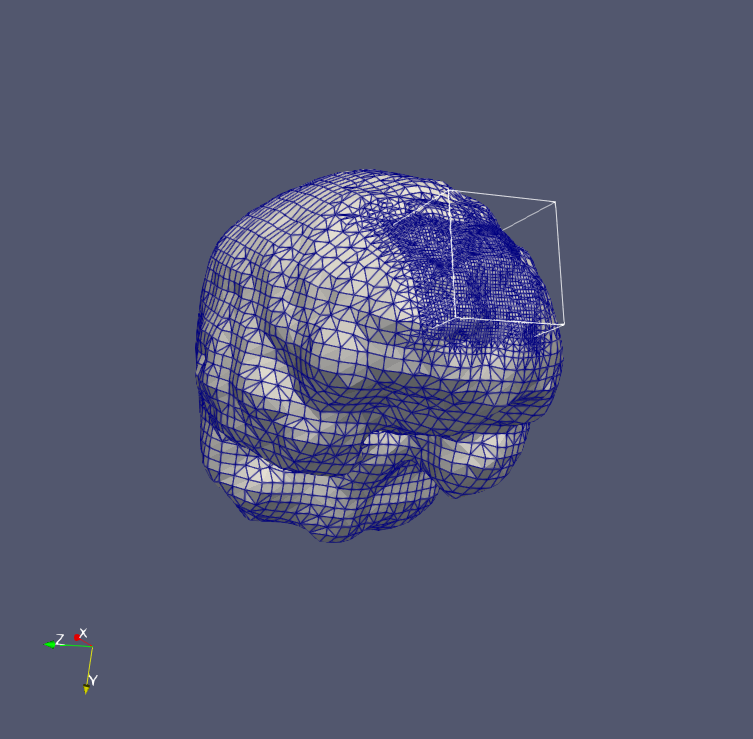
\includegraphics[width=1.0\textwidth]{figures/meshes/c_5r7_01.png}
        \caption{Zoom out de sección extraída.}
    \end{subfigure}
    \begin{subfigure}[t]{0.45\textwidth}
        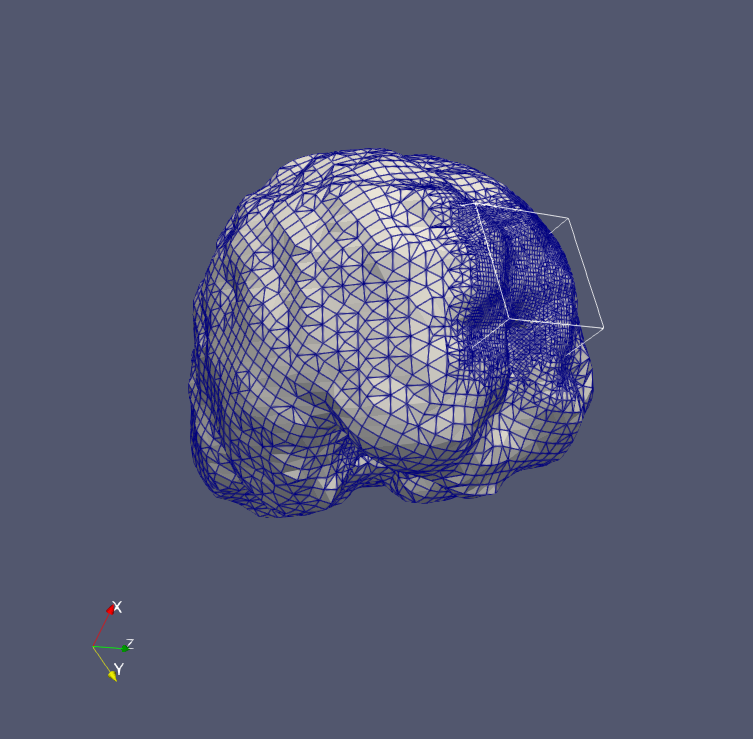
\includegraphics[width=1.0\textwidth]{figures/meshes/c_5r7_2_01.png}
        \caption{Zona extraída con elementos de mala calidad resaltados.}
    \end{subfigure}
    \caption{ Zona a analizar para evidenciar elementos de mala calidad, esta zona se extrajo de la representación de la malla con un nivel 5 de refinamiento general y nivel 7 de refinamiento en la superficie entregada. En la imagen de la izquierda se muestra una visión general de la superficie de la malla demarcada por elementos con vértices azules y la zona a estudiar de color celeste. En la imagen de la derecha, la zona a estudiar y un par de elementos de mala calidad destacados con color verde. }
    Fuente: Elaboración propia.
    \label{fig:zoom_cortex_surf}
\end{figure}



\begin{figure}[!ht]
    \centering
    \begin{subfigure}[t]{0.8\textwidth}
        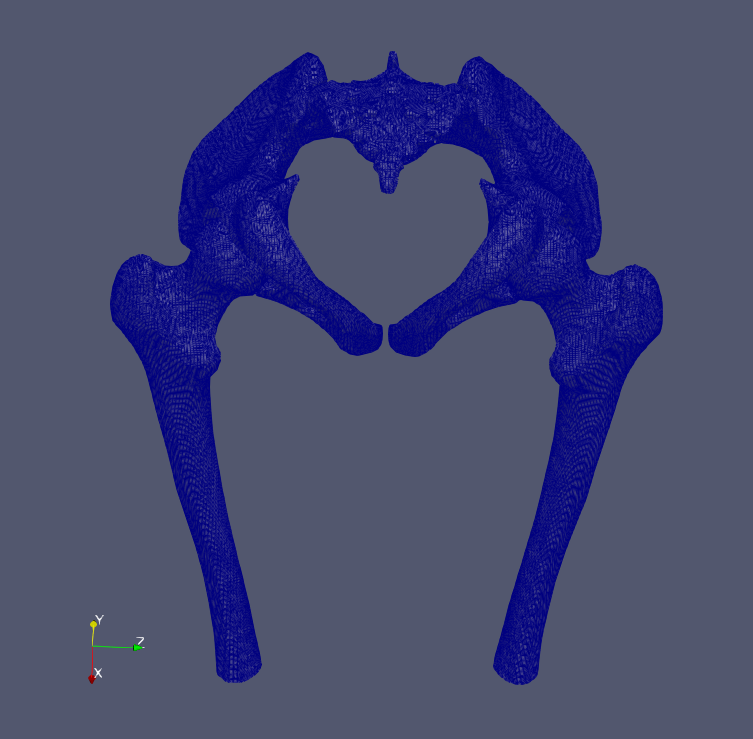
\includegraphics[width=1.0\textwidth]{figures/meshes/coxis_8r9_01.png}
        \caption{Zoom out de sección extraída.}
    \end{subfigure}
    \caption{ Zona a analizar para evidenciar elementos de mala calidad, esta zona se extrajo de la representación de la malla con un nivel 5 de refinamiento general y nivel 7 de refinamiento en la superficie entregada. En la imagen de la izquierda se muestra una visión general de la superficie de la malla demarcada por elementos con vértices azules y la zona a estudiar de color celeste. En la imagen de la derecha, la zona a estudiar y un par de elementos de mala calidad destacados con color verde. }
    Fuente: Elaboración propia.
    \label{fig:zoom_cortex_surf}
\end{figure}

\begin{figure}[!ht]
    \centering
    \begin{subfigure}[t]{0.45\textwidth}
        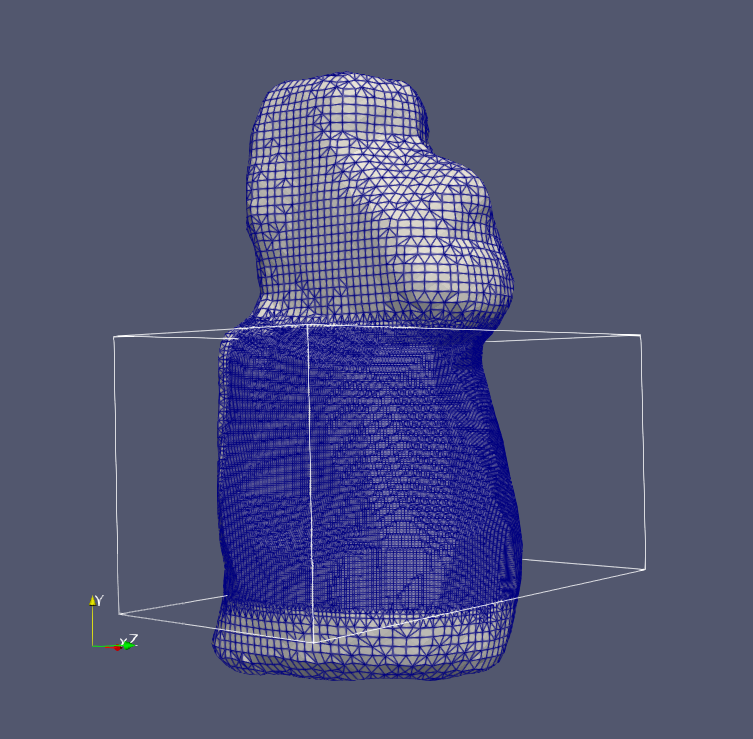
\includegraphics[width=1.0\textwidth]{figures/meshes/moai_5r7_01.png}
        \caption{Zoom out de sección extraída.}
    \end{subfigure}
    \begin{subfigure}[t]{0.45\textwidth}
        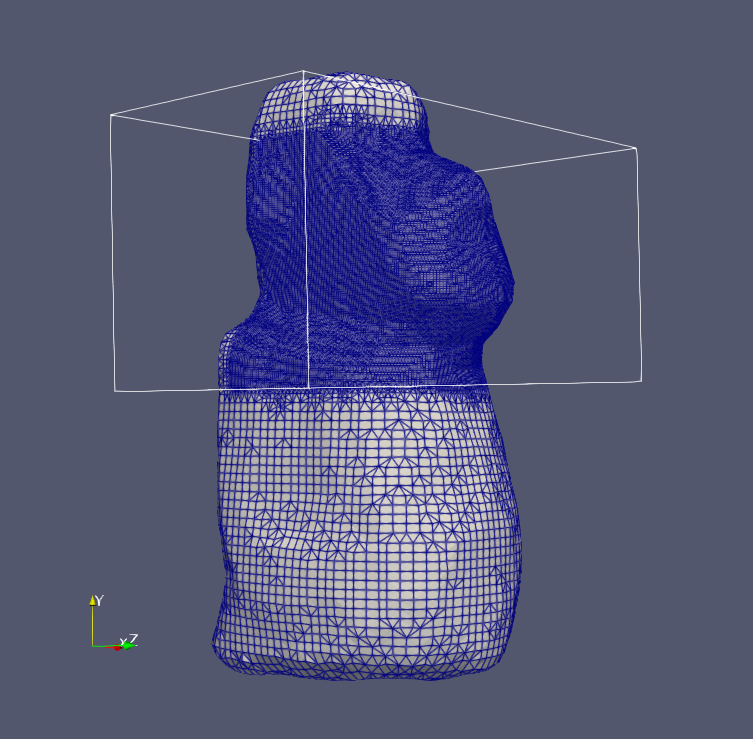
\includegraphics[width=1.0\textwidth]{figures/meshes/moai_5r7_2_01.png}
        \caption{Zona extraída con elementos de mala calidad resaltados.}
    \end{subfigure}
    \caption{ Zona a analizar para evidenciar elementos de mala calidad, esta zona se extrajo de la representación de la malla con un nivel 5 de refinamiento general y nivel 7 de refinamiento en la superficie entregada. En la imagen de la izquierda se muestra una visión general de la superficie de la malla demarcada por elementos con vértices azules y la zona a estudiar de color celeste. En la imagen de la derecha, la zona a estudiar y un par de elementos de mala calidad destacados con color verde. }
    Fuente: Elaboración propia.
    \label{fig:zoom_cortex_surf}
\end{figure}


\begin{figure}[!ht]
    \centering
    \begin{subfigure}[t]{0.8\textwidth}
        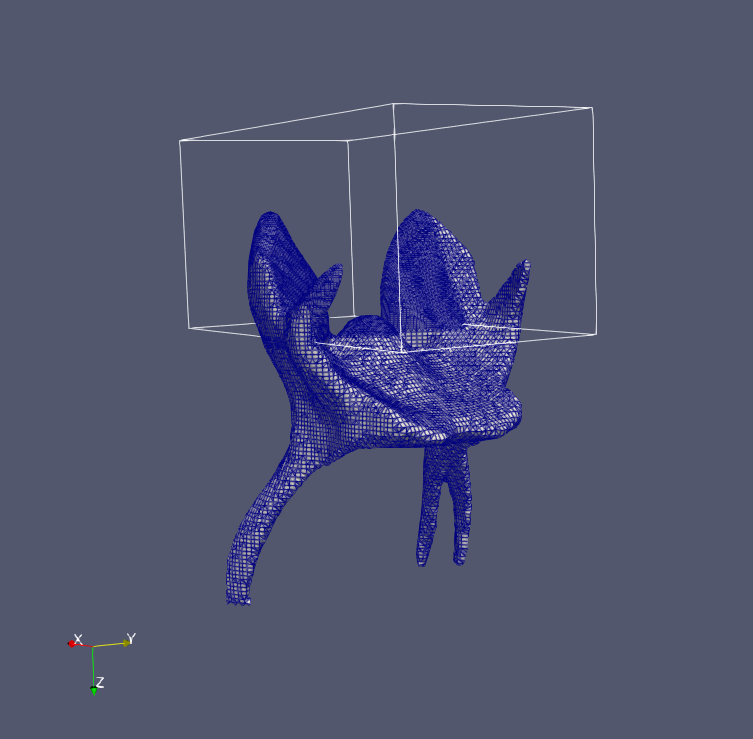
\includegraphics[width=1.0\textwidth]{figures/meshes/palate_5r7_01.png}
        \caption{Zoom out de sección extraída.}
    \end{subfigure}
    \caption{ Zona a analizar para evidenciar elementos de mala calidad, esta zona se extrajo de la representación de la malla con un nivel 5 de refinamiento general y nivel 7 de refinamiento en la superficie entregada. En la imagen de la izquierda se muestra una visión general de la superficie de la malla demarcada por elementos con vértices azules y la zona a estudiar de color celeste. En la imagen de la derecha, la zona a estudiar y un par de elementos de mala calidad destacados con color verde. }
    Fuente: Elaboración propia.
    \label{fig:zoom_cortex_surf}
\end{figure}
 \newpage
 \secnumbersection{Conclusiones}


%Las Conclusiones son, según algunos especialistas, el aspecto principal de una memoria, ya que reflejan el aprendizaje final del autor del documento. En ellas se tiende a considerar los alcances y limitaciones de la propuesta de solución, establecer de forma simple y directa los resultados, discutir respecto a la validez de los objetivos formulados, identificar las principales contribuciones y aplicaciones del trabajo realizado, así como su impacto o aporte a la organización o a los actores involucrados. Otro aspecto que tiende a incluirse son recomendaciones para quienes se sientan motivados por el tema y deseen profundizarlo, o lineamientos de una futura ampliación del trabajo.

%\underline{Todo esto debe sintetizarse en al menos 5 páginas.}

El algoritmo propuesto fue capaz de eliminar Elementos inválidos en la mayoría de los casos, sin modificar o provocar estiramiento en los nodos de la representación ni empobrecimiento de la calidad.

Al realizar la validación del algoritmo, solo una de las instancias de prueba falló. Cuando se utilizó diversos umbrales de calidad y regiones de interés, no hubo cambios considerables en el comportamiento del algoritmo ni degradación en las estadísticas $J_{ENS}$.

Si bien los tiempos no son óptimos considerando la complejidad del algoritmo, se logró el objetivo de este estudio, implementar y validar el algoritmo propuesto, no así la implementación.

Se recomienda, fijar la cantidad de iteraciones en 10, ya que, la mayoría de los casos se obtuvieron mallas válidas en a lo más 7 iteraciones. Cuando requería más iteraciones, las pruebas normalmente fallaban, como en el caso de la representación del Coxis, que diverge y genera mallas de peor calidad.



Por tanto, agregar una condición de término que realice el seguimiento del deterioro de la calidad de la malla y retorno automatizado a un estado anterior, es fundamental para casos como el ``moai\_5\_5r5\_1\_n'' registrado en \autoref{fig:bar_moai_all}. Aquí se muestra un posible punto intermedio en la iteración 8, dónde se logran cero \elements{} inválidos y dos \elements{} en $E_0^{0.03}$ y uno en $E_0^{0.05}$, una calidad aceptable para un threshold $0.05$. 


% TODO: optimizar la implementación 
	- no leer archivos con modelo de ddatos en cada iteración
	- no escribir en cada iteración las representaciones gráficas de las mallas, sólo hacerlo en la malla final
	
	
% TODO: proponer un sistema de software que gestione algoritmos iterativos, muestre el historial de las estadisticas de calidad y ayude al usuario a seccionar el mejor.

intro

	objetivos
	porqué

discusión sobre los resultados
qué siginifico para mi (proceso de implementacion)
lista problemas no resueltos o complejidades de la solucion

% TODO: considerar caso de coxis
% TODO: considerar limitación de tratamiento del modelo entre iteraciones, integrar todo en un proceso para no realizar lectura de archivos durante la iteracion del algoritmo.
% TODO: utilización malla cortex como caso simple y coxis como caso complejo para validar algoritmos futuros, estandarizar.
% TODO:  agregar una condicion de termino y retorno automatizado a un estado anterior.
% TODO: proponer un sistema de refinamiento local, es decir, que no itere toda la malla para encontrar un elemento u octante, sino que refine un octante y sólo modifique los octantes adyacentes o directamente conectados. Esto permitiría un refinamiento concurrente.

mejoras	
priorizacion del trabajo futuro



 \newpage
 \secnumberlesssection{ANEXOS}

En los Anexos se incluye todo aquel material complementario que no es parte del contenido de los capítulos de la memoria, pero que permiten a un lector contar con un contenido adjunto relacionado con el tema.


\newpage
% Bibliografía estilo APA:
\bibliographystyle{apalike-es}
\bibliography{bibliografia}{}

\end{document}
